
% Default to the notebook output style

    


% Inherit from the specified cell style.




    
\documentclass[11pt]{article}

    
    
    \usepackage[T1]{fontenc}
    % Nicer default font (+ math font) than Computer Modern for most use cases
    \usepackage{mathpazo}

    % Basic figure setup, for now with no caption control since it's done
    % automatically by Pandoc (which extracts ![](path) syntax from Markdown).
    \usepackage{graphicx}
    % We will generate all images so they have a width \maxwidth. This means
    % that they will get their normal width if they fit onto the page, but
    % are scaled down if they would overflow the margins.
    \makeatletter
    \def\maxwidth{\ifdim\Gin@nat@width>\linewidth\linewidth
    \else\Gin@nat@width\fi}
    \makeatother
    \let\Oldincludegraphics\includegraphics
    % Set max figure width to be 80% of text width, for now hardcoded.
    \renewcommand{\includegraphics}[1]{\Oldincludegraphics[width=.8\maxwidth]{#1}}
    % Ensure that by default, figures have no caption (until we provide a
    % proper Figure object with a Caption API and a way to capture that
    % in the conversion process - todo).
    \usepackage{caption}
    \DeclareCaptionLabelFormat{nolabel}{}
    \captionsetup{labelformat=nolabel}

    \usepackage{adjustbox} % Used to constrain images to a maximum size 
    \usepackage{xcolor} % Allow colors to be defined
    \usepackage{enumerate} % Needed for markdown enumerations to work
    \usepackage{geometry} % Used to adjust the document margins
    \usepackage{amsmath} % Equations
    \usepackage{amssymb} % Equations
    \usepackage{textcomp} % defines textquotesingle
    % Hack from http://tex.stackexchange.com/a/47451/13684:
    \AtBeginDocument{%
        \def\PYZsq{\textquotesingle}% Upright quotes in Pygmentized code
    }
    \usepackage{upquote} % Upright quotes for verbatim code
    \usepackage{eurosym} % defines \euro
    \usepackage[mathletters]{ucs} % Extended unicode (utf-8) support
    \usepackage[utf8x]{inputenc} % Allow utf-8 characters in the tex document
    \usepackage{fancyvrb} % verbatim replacement that allows latex
    \usepackage{grffile} % extends the file name processing of package graphics 
                         % to support a larger range 
    % The hyperref package gives us a pdf with properly built
    % internal navigation ('pdf bookmarks' for the table of contents,
    % internal cross-reference links, web links for URLs, etc.)
    \usepackage{hyperref}
    \usepackage{longtable} % longtable support required by pandoc >1.10
    \usepackage{booktabs}  % table support for pandoc > 1.12.2
    \usepackage[inline]{enumitem} % IRkernel/repr support (it uses the enumerate* environment)
    \usepackage[normalem]{ulem} % ulem is needed to support strikethroughs (\sout)
                                % normalem makes italics be italics, not underlines
    

    
    
    % Colors for the hyperref package
    \definecolor{urlcolor}{rgb}{0,.145,.698}
    \definecolor{linkcolor}{rgb}{.71,0.21,0.01}
    \definecolor{citecolor}{rgb}{.12,.54,.11}

    % ANSI colors
    \definecolor{ansi-black}{HTML}{3E424D}
    \definecolor{ansi-black-intense}{HTML}{282C36}
    \definecolor{ansi-red}{HTML}{E75C58}
    \definecolor{ansi-red-intense}{HTML}{B22B31}
    \definecolor{ansi-green}{HTML}{00A250}
    \definecolor{ansi-green-intense}{HTML}{007427}
    \definecolor{ansi-yellow}{HTML}{DDB62B}
    \definecolor{ansi-yellow-intense}{HTML}{B27D12}
    \definecolor{ansi-blue}{HTML}{208FFB}
    \definecolor{ansi-blue-intense}{HTML}{0065CA}
    \definecolor{ansi-magenta}{HTML}{D160C4}
    \definecolor{ansi-magenta-intense}{HTML}{A03196}
    \definecolor{ansi-cyan}{HTML}{60C6C8}
    \definecolor{ansi-cyan-intense}{HTML}{258F8F}
    \definecolor{ansi-white}{HTML}{C5C1B4}
    \definecolor{ansi-white-intense}{HTML}{A1A6B2}

    % commands and environments needed by pandoc snippets
    % extracted from the output of `pandoc -s`
    \providecommand{\tightlist}{%
      \setlength{\itemsep}{0pt}\setlength{\parskip}{0pt}}
    \DefineVerbatimEnvironment{Highlighting}{Verbatim}{commandchars=\\\{\}}
    % Add ',fontsize=\small' for more characters per line
    \newenvironment{Shaded}{}{}
    \newcommand{\KeywordTok}[1]{\textcolor[rgb]{0.00,0.44,0.13}{\textbf{{#1}}}}
    \newcommand{\DataTypeTok}[1]{\textcolor[rgb]{0.56,0.13,0.00}{{#1}}}
    \newcommand{\DecValTok}[1]{\textcolor[rgb]{0.25,0.63,0.44}{{#1}}}
    \newcommand{\BaseNTok}[1]{\textcolor[rgb]{0.25,0.63,0.44}{{#1}}}
    \newcommand{\FloatTok}[1]{\textcolor[rgb]{0.25,0.63,0.44}{{#1}}}
    \newcommand{\CharTok}[1]{\textcolor[rgb]{0.25,0.44,0.63}{{#1}}}
    \newcommand{\StringTok}[1]{\textcolor[rgb]{0.25,0.44,0.63}{{#1}}}
    \newcommand{\CommentTok}[1]{\textcolor[rgb]{0.38,0.63,0.69}{\textit{{#1}}}}
    \newcommand{\OtherTok}[1]{\textcolor[rgb]{0.00,0.44,0.13}{{#1}}}
    \newcommand{\AlertTok}[1]{\textcolor[rgb]{1.00,0.00,0.00}{\textbf{{#1}}}}
    \newcommand{\FunctionTok}[1]{\textcolor[rgb]{0.02,0.16,0.49}{{#1}}}
    \newcommand{\RegionMarkerTok}[1]{{#1}}
    \newcommand{\ErrorTok}[1]{\textcolor[rgb]{1.00,0.00,0.00}{\textbf{{#1}}}}
    \newcommand{\NormalTok}[1]{{#1}}
    
    % Additional commands for more recent versions of Pandoc
    \newcommand{\ConstantTok}[1]{\textcolor[rgb]{0.53,0.00,0.00}{{#1}}}
    \newcommand{\SpecialCharTok}[1]{\textcolor[rgb]{0.25,0.44,0.63}{{#1}}}
    \newcommand{\VerbatimStringTok}[1]{\textcolor[rgb]{0.25,0.44,0.63}{{#1}}}
    \newcommand{\SpecialStringTok}[1]{\textcolor[rgb]{0.73,0.40,0.53}{{#1}}}
    \newcommand{\ImportTok}[1]{{#1}}
    \newcommand{\DocumentationTok}[1]{\textcolor[rgb]{0.73,0.13,0.13}{\textit{{#1}}}}
    \newcommand{\AnnotationTok}[1]{\textcolor[rgb]{0.38,0.63,0.69}{\textbf{\textit{{#1}}}}}
    \newcommand{\CommentVarTok}[1]{\textcolor[rgb]{0.38,0.63,0.69}{\textbf{\textit{{#1}}}}}
    \newcommand{\VariableTok}[1]{\textcolor[rgb]{0.10,0.09,0.49}{{#1}}}
    \newcommand{\ControlFlowTok}[1]{\textcolor[rgb]{0.00,0.44,0.13}{\textbf{{#1}}}}
    \newcommand{\OperatorTok}[1]{\textcolor[rgb]{0.40,0.40,0.40}{{#1}}}
    \newcommand{\BuiltInTok}[1]{{#1}}
    \newcommand{\ExtensionTok}[1]{{#1}}
    \newcommand{\PreprocessorTok}[1]{\textcolor[rgb]{0.74,0.48,0.00}{{#1}}}
    \newcommand{\AttributeTok}[1]{\textcolor[rgb]{0.49,0.56,0.16}{{#1}}}
    \newcommand{\InformationTok}[1]{\textcolor[rgb]{0.38,0.63,0.69}{\textbf{\textit{{#1}}}}}
    \newcommand{\WarningTok}[1]{\textcolor[rgb]{0.38,0.63,0.69}{\textbf{\textit{{#1}}}}}
    
    
    % Define a nice break command that doesn't care if a line doesn't already
    % exist.
    \def\br{\hspace*{\fill} \\* }
    % Math Jax compatability definitions
    \def\gt{>}
    \def\lt{<}
    % Document parameters
    \title{DIP-HW3}
    
    
    

    % Pygments definitions
    
\makeatletter
\def\PY@reset{\let\PY@it=\relax \let\PY@bf=\relax%
    \let\PY@ul=\relax \let\PY@tc=\relax%
    \let\PY@bc=\relax \let\PY@ff=\relax}
\def\PY@tok#1{\csname PY@tok@#1\endcsname}
\def\PY@toks#1+{\ifx\relax#1\empty\else%
    \PY@tok{#1}\expandafter\PY@toks\fi}
\def\PY@do#1{\PY@bc{\PY@tc{\PY@ul{%
    \PY@it{\PY@bf{\PY@ff{#1}}}}}}}
\def\PY#1#2{\PY@reset\PY@toks#1+\relax+\PY@do{#2}}

\expandafter\def\csname PY@tok@w\endcsname{\def\PY@tc##1{\textcolor[rgb]{0.73,0.73,0.73}{##1}}}
\expandafter\def\csname PY@tok@c\endcsname{\let\PY@it=\textit\def\PY@tc##1{\textcolor[rgb]{0.25,0.50,0.50}{##1}}}
\expandafter\def\csname PY@tok@cp\endcsname{\def\PY@tc##1{\textcolor[rgb]{0.74,0.48,0.00}{##1}}}
\expandafter\def\csname PY@tok@k\endcsname{\let\PY@bf=\textbf\def\PY@tc##1{\textcolor[rgb]{0.00,0.50,0.00}{##1}}}
\expandafter\def\csname PY@tok@kp\endcsname{\def\PY@tc##1{\textcolor[rgb]{0.00,0.50,0.00}{##1}}}
\expandafter\def\csname PY@tok@kt\endcsname{\def\PY@tc##1{\textcolor[rgb]{0.69,0.00,0.25}{##1}}}
\expandafter\def\csname PY@tok@o\endcsname{\def\PY@tc##1{\textcolor[rgb]{0.40,0.40,0.40}{##1}}}
\expandafter\def\csname PY@tok@ow\endcsname{\let\PY@bf=\textbf\def\PY@tc##1{\textcolor[rgb]{0.67,0.13,1.00}{##1}}}
\expandafter\def\csname PY@tok@nb\endcsname{\def\PY@tc##1{\textcolor[rgb]{0.00,0.50,0.00}{##1}}}
\expandafter\def\csname PY@tok@nf\endcsname{\def\PY@tc##1{\textcolor[rgb]{0.00,0.00,1.00}{##1}}}
\expandafter\def\csname PY@tok@nc\endcsname{\let\PY@bf=\textbf\def\PY@tc##1{\textcolor[rgb]{0.00,0.00,1.00}{##1}}}
\expandafter\def\csname PY@tok@nn\endcsname{\let\PY@bf=\textbf\def\PY@tc##1{\textcolor[rgb]{0.00,0.00,1.00}{##1}}}
\expandafter\def\csname PY@tok@ne\endcsname{\let\PY@bf=\textbf\def\PY@tc##1{\textcolor[rgb]{0.82,0.25,0.23}{##1}}}
\expandafter\def\csname PY@tok@nv\endcsname{\def\PY@tc##1{\textcolor[rgb]{0.10,0.09,0.49}{##1}}}
\expandafter\def\csname PY@tok@no\endcsname{\def\PY@tc##1{\textcolor[rgb]{0.53,0.00,0.00}{##1}}}
\expandafter\def\csname PY@tok@nl\endcsname{\def\PY@tc##1{\textcolor[rgb]{0.63,0.63,0.00}{##1}}}
\expandafter\def\csname PY@tok@ni\endcsname{\let\PY@bf=\textbf\def\PY@tc##1{\textcolor[rgb]{0.60,0.60,0.60}{##1}}}
\expandafter\def\csname PY@tok@na\endcsname{\def\PY@tc##1{\textcolor[rgb]{0.49,0.56,0.16}{##1}}}
\expandafter\def\csname PY@tok@nt\endcsname{\let\PY@bf=\textbf\def\PY@tc##1{\textcolor[rgb]{0.00,0.50,0.00}{##1}}}
\expandafter\def\csname PY@tok@nd\endcsname{\def\PY@tc##1{\textcolor[rgb]{0.67,0.13,1.00}{##1}}}
\expandafter\def\csname PY@tok@s\endcsname{\def\PY@tc##1{\textcolor[rgb]{0.73,0.13,0.13}{##1}}}
\expandafter\def\csname PY@tok@sd\endcsname{\let\PY@it=\textit\def\PY@tc##1{\textcolor[rgb]{0.73,0.13,0.13}{##1}}}
\expandafter\def\csname PY@tok@si\endcsname{\let\PY@bf=\textbf\def\PY@tc##1{\textcolor[rgb]{0.73,0.40,0.53}{##1}}}
\expandafter\def\csname PY@tok@se\endcsname{\let\PY@bf=\textbf\def\PY@tc##1{\textcolor[rgb]{0.73,0.40,0.13}{##1}}}
\expandafter\def\csname PY@tok@sr\endcsname{\def\PY@tc##1{\textcolor[rgb]{0.73,0.40,0.53}{##1}}}
\expandafter\def\csname PY@tok@ss\endcsname{\def\PY@tc##1{\textcolor[rgb]{0.10,0.09,0.49}{##1}}}
\expandafter\def\csname PY@tok@sx\endcsname{\def\PY@tc##1{\textcolor[rgb]{0.00,0.50,0.00}{##1}}}
\expandafter\def\csname PY@tok@m\endcsname{\def\PY@tc##1{\textcolor[rgb]{0.40,0.40,0.40}{##1}}}
\expandafter\def\csname PY@tok@gh\endcsname{\let\PY@bf=\textbf\def\PY@tc##1{\textcolor[rgb]{0.00,0.00,0.50}{##1}}}
\expandafter\def\csname PY@tok@gu\endcsname{\let\PY@bf=\textbf\def\PY@tc##1{\textcolor[rgb]{0.50,0.00,0.50}{##1}}}
\expandafter\def\csname PY@tok@gd\endcsname{\def\PY@tc##1{\textcolor[rgb]{0.63,0.00,0.00}{##1}}}
\expandafter\def\csname PY@tok@gi\endcsname{\def\PY@tc##1{\textcolor[rgb]{0.00,0.63,0.00}{##1}}}
\expandafter\def\csname PY@tok@gr\endcsname{\def\PY@tc##1{\textcolor[rgb]{1.00,0.00,0.00}{##1}}}
\expandafter\def\csname PY@tok@ge\endcsname{\let\PY@it=\textit}
\expandafter\def\csname PY@tok@gs\endcsname{\let\PY@bf=\textbf}
\expandafter\def\csname PY@tok@gp\endcsname{\let\PY@bf=\textbf\def\PY@tc##1{\textcolor[rgb]{0.00,0.00,0.50}{##1}}}
\expandafter\def\csname PY@tok@go\endcsname{\def\PY@tc##1{\textcolor[rgb]{0.53,0.53,0.53}{##1}}}
\expandafter\def\csname PY@tok@gt\endcsname{\def\PY@tc##1{\textcolor[rgb]{0.00,0.27,0.87}{##1}}}
\expandafter\def\csname PY@tok@err\endcsname{\def\PY@bc##1{\setlength{\fboxsep}{0pt}\fcolorbox[rgb]{1.00,0.00,0.00}{1,1,1}{\strut ##1}}}
\expandafter\def\csname PY@tok@kc\endcsname{\let\PY@bf=\textbf\def\PY@tc##1{\textcolor[rgb]{0.00,0.50,0.00}{##1}}}
\expandafter\def\csname PY@tok@kd\endcsname{\let\PY@bf=\textbf\def\PY@tc##1{\textcolor[rgb]{0.00,0.50,0.00}{##1}}}
\expandafter\def\csname PY@tok@kn\endcsname{\let\PY@bf=\textbf\def\PY@tc##1{\textcolor[rgb]{0.00,0.50,0.00}{##1}}}
\expandafter\def\csname PY@tok@kr\endcsname{\let\PY@bf=\textbf\def\PY@tc##1{\textcolor[rgb]{0.00,0.50,0.00}{##1}}}
\expandafter\def\csname PY@tok@bp\endcsname{\def\PY@tc##1{\textcolor[rgb]{0.00,0.50,0.00}{##1}}}
\expandafter\def\csname PY@tok@fm\endcsname{\def\PY@tc##1{\textcolor[rgb]{0.00,0.00,1.00}{##1}}}
\expandafter\def\csname PY@tok@vc\endcsname{\def\PY@tc##1{\textcolor[rgb]{0.10,0.09,0.49}{##1}}}
\expandafter\def\csname PY@tok@vg\endcsname{\def\PY@tc##1{\textcolor[rgb]{0.10,0.09,0.49}{##1}}}
\expandafter\def\csname PY@tok@vi\endcsname{\def\PY@tc##1{\textcolor[rgb]{0.10,0.09,0.49}{##1}}}
\expandafter\def\csname PY@tok@vm\endcsname{\def\PY@tc##1{\textcolor[rgb]{0.10,0.09,0.49}{##1}}}
\expandafter\def\csname PY@tok@sa\endcsname{\def\PY@tc##1{\textcolor[rgb]{0.73,0.13,0.13}{##1}}}
\expandafter\def\csname PY@tok@sb\endcsname{\def\PY@tc##1{\textcolor[rgb]{0.73,0.13,0.13}{##1}}}
\expandafter\def\csname PY@tok@sc\endcsname{\def\PY@tc##1{\textcolor[rgb]{0.73,0.13,0.13}{##1}}}
\expandafter\def\csname PY@tok@dl\endcsname{\def\PY@tc##1{\textcolor[rgb]{0.73,0.13,0.13}{##1}}}
\expandafter\def\csname PY@tok@s2\endcsname{\def\PY@tc##1{\textcolor[rgb]{0.73,0.13,0.13}{##1}}}
\expandafter\def\csname PY@tok@sh\endcsname{\def\PY@tc##1{\textcolor[rgb]{0.73,0.13,0.13}{##1}}}
\expandafter\def\csname PY@tok@s1\endcsname{\def\PY@tc##1{\textcolor[rgb]{0.73,0.13,0.13}{##1}}}
\expandafter\def\csname PY@tok@mb\endcsname{\def\PY@tc##1{\textcolor[rgb]{0.40,0.40,0.40}{##1}}}
\expandafter\def\csname PY@tok@mf\endcsname{\def\PY@tc##1{\textcolor[rgb]{0.40,0.40,0.40}{##1}}}
\expandafter\def\csname PY@tok@mh\endcsname{\def\PY@tc##1{\textcolor[rgb]{0.40,0.40,0.40}{##1}}}
\expandafter\def\csname PY@tok@mi\endcsname{\def\PY@tc##1{\textcolor[rgb]{0.40,0.40,0.40}{##1}}}
\expandafter\def\csname PY@tok@il\endcsname{\def\PY@tc##1{\textcolor[rgb]{0.40,0.40,0.40}{##1}}}
\expandafter\def\csname PY@tok@mo\endcsname{\def\PY@tc##1{\textcolor[rgb]{0.40,0.40,0.40}{##1}}}
\expandafter\def\csname PY@tok@ch\endcsname{\let\PY@it=\textit\def\PY@tc##1{\textcolor[rgb]{0.25,0.50,0.50}{##1}}}
\expandafter\def\csname PY@tok@cm\endcsname{\let\PY@it=\textit\def\PY@tc##1{\textcolor[rgb]{0.25,0.50,0.50}{##1}}}
\expandafter\def\csname PY@tok@cpf\endcsname{\let\PY@it=\textit\def\PY@tc##1{\textcolor[rgb]{0.25,0.50,0.50}{##1}}}
\expandafter\def\csname PY@tok@c1\endcsname{\let\PY@it=\textit\def\PY@tc##1{\textcolor[rgb]{0.25,0.50,0.50}{##1}}}
\expandafter\def\csname PY@tok@cs\endcsname{\let\PY@it=\textit\def\PY@tc##1{\textcolor[rgb]{0.25,0.50,0.50}{##1}}}

\def\PYZbs{\char`\\}
\def\PYZus{\char`\_}
\def\PYZob{\char`\{}
\def\PYZcb{\char`\}}
\def\PYZca{\char`\^}
\def\PYZam{\char`\&}
\def\PYZlt{\char`\<}
\def\PYZgt{\char`\>}
\def\PYZsh{\char`\#}
\def\PYZpc{\char`\%}
\def\PYZdl{\char`\$}
\def\PYZhy{\char`\-}
\def\PYZsq{\char`\'}
\def\PYZdq{\char`\"}
\def\PYZti{\char`\~}
% for compatibility with earlier versions
\def\PYZat{@}
\def\PYZlb{[}
\def\PYZrb{]}
\makeatother


    % Exact colors from NB
    \definecolor{incolor}{rgb}{0.0, 0.0, 0.5}
    \definecolor{outcolor}{rgb}{0.545, 0.0, 0.0}



    
    % Prevent overflowing lines due to hard-to-break entities
    \sloppy 
    % Setup hyperref package
    \hypersetup{
      breaklinks=true,  % so long urls are correctly broken across lines
      colorlinks=true,
      urlcolor=urlcolor,
      linkcolor=linkcolor,
      citecolor=citecolor,
      }
    % Slightly bigger margins than the latex defaults
    
    \geometry{verbose,tmargin=1in,bmargin=1in,lmargin=1in,rmargin=1in}
    
    

    \begin{document}
    
    
    \maketitle
    
    

    
    \hypertarget{digital-image-processing---hw3---98722278---mohammad-doosti-lakhani}{%
\section{Digital Image Processing - HW3 - 98722278 - Mohammad Doosti
Lakhani}\label{digital-image-processing---hw3---98722278---mohammad-doosti-lakhani}}

In this notebook, I have solved the assignment's problems which are as
follows:

\begin{enumerate}
\def\labelenumi{\arabic{enumi}.}
\tightlist
\item
  In the below images (left), vertical black and white strips with 2
  pixel width exists. The image on the right indicates its frequency
  spectrum. Answer the following questions about the given information:

  \begin{enumerate}
  \def\labelenumii{\arabic{enumii}.}
  \tightlist
  \item
    Why frequency spectrum only exists in \textbf{horizontal} dimension?
  \item
    If the width of strips increase to \textbf{4 pixel}, how will the
    frequency spectrum change?
  \item
    If the width of strips increase to \textbf{1 pixel}, how will the
    frequency spectrum change?
  \item
    If we use \textbf{DCT} instead of \textbf{DFT}, what will be the
    differences in frequency spectrum?
  \end{enumerate}
\end{enumerate}

\begin{figure}
\centering

\includegraphics{wiki/q01.jpg}
\caption{vertical strips image and its DFT transform}
\end{figure}

\begin{enumerate}
\def\labelenumi{\arabic{enumi}.}
\setcounter{enumi}{1}
\tightlist
\item
  Do the following tasks on \texttt{image2} and \texttt{image3}:

  \begin{enumerate}
  \def\labelenumii{\arabic{enumii}.}
  \tightlist
  \item
    Use available functions to calculate 2D \texttt{DFT} and
    \texttt{DCT} and show the results.
  \item
    For both of the \texttt{DCT} and \texttt{DFT} transforms, sort the
    absolute value of their factors. Also, Sort the brighness values of
    the images.
  \item
    Calculate the squared cumulutive sum of those values and plot those.
  \item
    Analyze the obtained results.
  \end{enumerate}
\item
  Do the following tasks on \texttt{striping.bmp} image:

  \begin{enumerate}
  \def\labelenumii{\arabic{enumii}.}
  \tightlist
  \item
    Reduce the noises in the \texttt{striping.bmp} image in \texttt{DCT}
    domain as much as possible without considerable decrease in image
    quality.
  \item
    Explain the procedure and demonstrate the result.
  \end{enumerate}
\item
  In the reference book, the process of achieving \texttt{DCT} using
  \texttt{FFT} for 1D has been explained. As \texttt{DCT} is a separable
  function, we can use the aforementioned approach to obtain the
  \texttt{DCT} in higher orders. So the tasks for this questions:

  \begin{enumerate}
  \def\labelenumii{\arabic{enumii}.}
  \tightlist
  \item
    Show the mathematical calculations to obtain the 2D \texttt{DCT}.
  \item
    Write a program to calculate \texttt{DCT} of an image using your
    approach.
  \item
    Apply your \texttt{DCT} function from step 2 on \texttt{image1.tif}
    and compare your result the one obtained from question 2.
  \end{enumerate}
\end{enumerate}

    \hypertarget{frequency-spectrum-of-dct-and-dft}{%
\subsection{1 Frequency Spectrum of DCT and
DFT}\label{frequency-spectrum-of-dct-and-dft}}

In the below images (left), vertical black and white strips with 2 pixel
width exists. The image on the right indicates its frequency spectrum.
Answer the following questions about the given information: 1. Why
frequency spectrum only exists in \textbf{horizontal} dimension? 2. If
the width of strips increase to \textbf{4 pixel}, how will the frequency
spectrum change? 3. If the width of strips increase to \textbf{1 pixel},
how will the frequency spectrum change? 4. If we use \textbf{DCT}
instead of \textbf{DFT}, what will be the differences in frequency
spectrum?


\includegraphics{wiki/q01.jpg}

    I try to answer all the questions in this section using following images
from \protect\hyperlink{}{Dr.~Mohammadi at Iran University of Science
and Technology - Instructor}:

DFT basic functions: 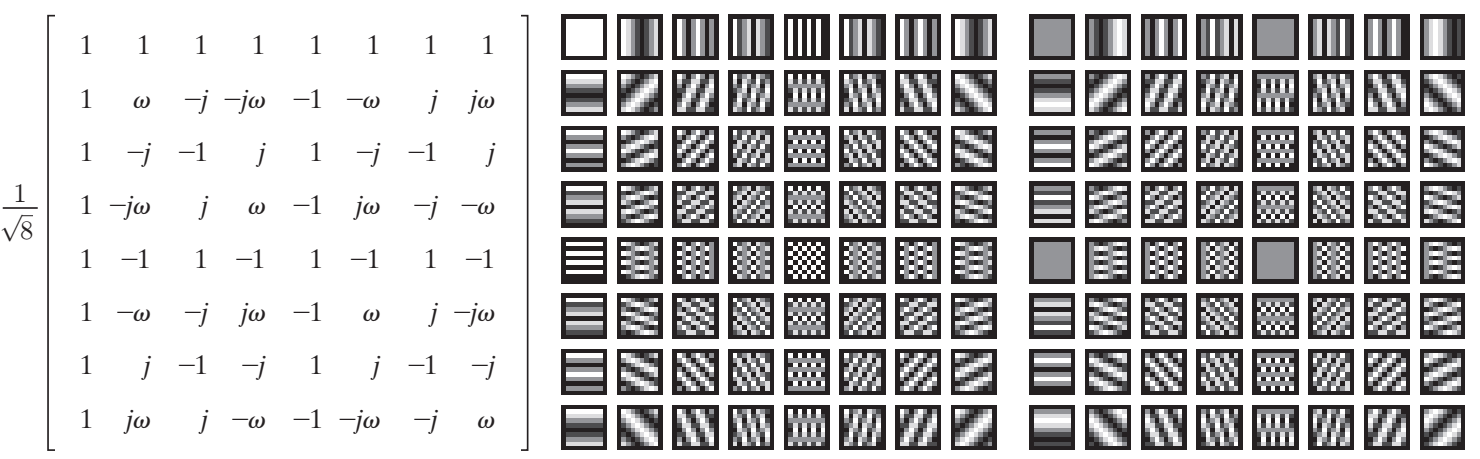
\includegraphics{wiki/dft-table.jpg}

DCT basic functions: 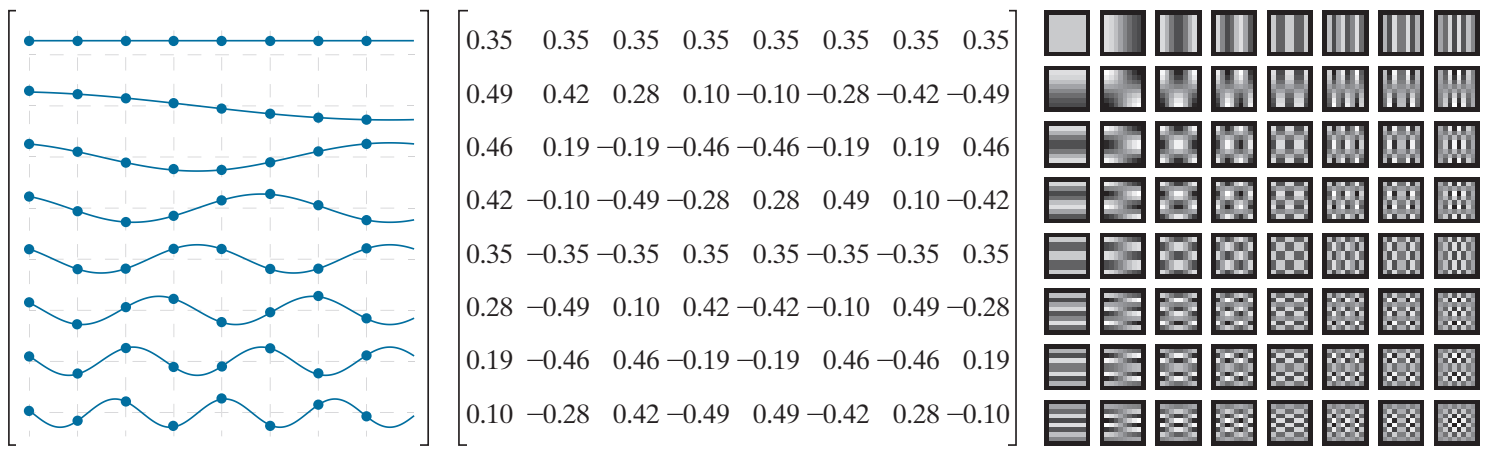
\includegraphics{wiki/dct-table.jpg}

    \hypertarget{a-horizontal-values-for-vertical-strips}{%
\subsubsection{1.A Horizontal values for vertical
strips}\label{a-horizontal-values-for-vertical-strips}}

So as we can see in the DFT's basis functions, vertical strips exists in
horizontal dimension. Actually, we just need to compare first row and
first column and it is obvious that \textbf{vertical strips means
consistent change horizontally}, so first row is the functions that
representing the frequency spectrum of the given image. Furthermore, the
\textbf{DC} value, the pixel in the center of the frequency spectrum
will be light always in this question because we have a lot of pixels
with 255 value. Note: The images of basic functions are not shifted but
the image in the question is shifted.

    \begin{Verbatim}[commandchars=\\\{\}]
{\color{incolor}In [{\color{incolor}1}]:} \PY{k+kn}{import} \PY{n+nn}{numpy} \PY{k}{as} \PY{n+nn}{np}
        \PY{k+kn}{import} \PY{n+nn}{cv2}
        \PY{k+kn}{from} \PY{n+nn}{matplotlib} \PY{k}{import} \PY{n}{pyplot} \PY{k}{as} \PY{n}{plt}
        \PY{k+kn}{import} \PY{n+nn}{os}
        \PY{o}{\PYZpc{}}\PY{k}{matplotlib} inline
\end{Verbatim}


    \begin{Verbatim}[commandchars=\\\{\}]
{\color{incolor}In [{\color{incolor}10}]:} \PY{n}{image} \PY{o}{=} \PY{n}{np}\PY{o}{.}\PY{n}{zeros}\PY{p}{(}\PY{p}{(}\PY{l+m+mi}{8}\PY{p}{,} \PY{l+m+mi}{8}\PY{p}{)}\PY{p}{,} \PY{n}{dtype}\PY{o}{=}\PY{n}{np}\PY{o}{.}\PY{n}{int}\PY{p}{)}
         \PY{n}{image}\PY{p}{[}\PY{p}{:}\PY{p}{,}\PY{l+m+mi}{0}\PY{p}{:}\PY{p}{:}\PY{l+m+mi}{4}\PY{p}{]} \PY{o}{=} \PY{l+m+mi}{255}
         \PY{n}{image}\PY{p}{[}\PY{p}{:}\PY{p}{,}\PY{l+m+mi}{1}\PY{p}{:}\PY{p}{:}\PY{l+m+mi}{4}\PY{p}{]} \PY{o}{=} \PY{l+m+mi}{255}
         
         \PY{n}{f} \PY{o}{=} \PY{n}{np}\PY{o}{.}\PY{n}{fft}\PY{o}{.}\PY{n}{fft2}\PY{p}{(}\PY{n}{image}\PY{p}{)}
         \PY{n}{fshift} \PY{o}{=} \PY{n}{np}\PY{o}{.}\PY{n}{fft}\PY{o}{.}\PY{n}{fftshift}\PY{p}{(}\PY{n}{f}\PY{p}{)}
         
         \PY{n}{c} \PY{o}{=} \PY{n}{cv2}\PY{o}{.}\PY{n}{dct}\PY{p}{(}\PY{n}{np}\PY{o}{.}\PY{n}{float32}\PY{p}{(}\PY{n}{image}\PY{p}{)}\PY{p}{)}
         
         \PY{c+c1}{\PYZsh{} plot}
         \PY{n}{fig}\PY{p}{,} \PY{n}{ax} \PY{o}{=} \PY{n}{plt}\PY{o}{.}\PY{n}{subplots}\PY{p}{(}\PY{n}{nrows}\PY{o}{=}\PY{l+m+mi}{1}\PY{p}{,} \PY{n}{ncols}\PY{o}{=}\PY{l+m+mi}{3}\PY{p}{,} \PY{n}{figsize}\PY{o}{=}\PY{p}{(}\PY{l+m+mi}{20}\PY{p}{,} \PY{l+m+mi}{15}\PY{p}{)}\PY{p}{)}
         
         \PY{n}{ax}\PY{p}{[}\PY{l+m+mi}{0}\PY{p}{]}\PY{o}{.}\PY{n}{set\PYZus{}title}\PY{p}{(}\PY{l+s+s1}{\PYZsq{}}\PY{l+s+s1}{Original}\PY{l+s+s1}{\PYZsq{}}\PY{p}{)}
         \PY{n}{ax}\PY{p}{[}\PY{l+m+mi}{0}\PY{p}{]}\PY{o}{.}\PY{n}{imshow}\PY{p}{(}\PY{n}{image}\PY{p}{,} \PY{n}{cmap}\PY{o}{=}\PY{l+s+s1}{\PYZsq{}}\PY{l+s+s1}{gray}\PY{l+s+s1}{\PYZsq{}}\PY{p}{)}
         
         \PY{n}{ax}\PY{p}{[}\PY{l+m+mi}{1}\PY{p}{]}\PY{o}{.}\PY{n}{set\PYZus{}title}\PY{p}{(}\PY{l+s+s1}{\PYZsq{}}\PY{l+s+s1}{DFT}\PY{l+s+s1}{\PYZsq{}}\PY{p}{)}
         \PY{n}{ax}\PY{p}{[}\PY{l+m+mi}{1}\PY{p}{]}\PY{o}{.}\PY{n}{imshow}\PY{p}{(}\PY{n}{np}\PY{o}{.}\PY{n}{abs}\PY{p}{(}\PY{n}{fshift}\PY{p}{)}\PY{p}{,} \PY{n}{cmap} \PY{o}{=} \PY{l+s+s1}{\PYZsq{}}\PY{l+s+s1}{gray}\PY{l+s+s1}{\PYZsq{}}\PY{p}{)}
         
         \PY{n}{ax}\PY{p}{[}\PY{l+m+mi}{2}\PY{p}{]}\PY{o}{.}\PY{n}{set\PYZus{}title}\PY{p}{(}\PY{l+s+s1}{\PYZsq{}}\PY{l+s+s1}{DCT}\PY{l+s+s1}{\PYZsq{}}\PY{p}{)}
         \PY{n}{ax}\PY{p}{[}\PY{l+m+mi}{2}\PY{p}{]}\PY{o}{.}\PY{n}{imshow}\PY{p}{(}\PY{n}{c}\PY{p}{,} \PY{n}{cmap} \PY{o}{=} \PY{l+s+s1}{\PYZsq{}}\PY{l+s+s1}{gray}\PY{l+s+s1}{\PYZsq{}}\PY{p}{)}
\end{Verbatim}


\begin{Verbatim}[commandchars=\\\{\}]
{\color{outcolor}Out[{\color{outcolor}10}]:} <matplotlib.image.AxesImage at 0x24b6a357f98>
\end{Verbatim}
            
    \begin{center}
    \adjustimage{max size={0.9\linewidth}{0.9\paperheight}}{output_5_1.png}
    \end{center}
    { \hspace*{\fill} \\}
    
    \hypertarget{b-double-widths-of-strips}{%
\subsubsection{1.B Double Widths of
Strips}\label{b-double-widths-of-strips}}

We know that when the image is natural, there a few pixels that have
high frequency so almost all images concentrates on the center of the
DFT transform and as we increase the radius from the center to the
frame, the high frequency areas are covered so in this change, doubling
the strip sizes, we are reducing the amount of changes so basic
functions with less horizontal changes will have bigger factors and the
output image of DFT (frequency spectrum) will have more dense light
pixels. In other words, the functions that covers this kind of
frequencies are near to the center than before.

    \begin{Verbatim}[commandchars=\\\{\}]
{\color{incolor}In [{\color{incolor}14}]:} \PY{n}{image} \PY{o}{=} \PY{n}{np}\PY{o}{.}\PY{n}{zeros}\PY{p}{(}\PY{p}{(}\PY{l+m+mi}{8}\PY{p}{,} \PY{l+m+mi}{8}\PY{p}{)}\PY{p}{,} \PY{n}{dtype}\PY{o}{=}\PY{n}{np}\PY{o}{.}\PY{n}{int}\PY{p}{)}
         \PY{n}{image}\PY{p}{[}\PY{p}{:}\PY{p}{,}\PY{l+m+mi}{0}\PY{p}{:}\PY{p}{:}\PY{l+m+mi}{8}\PY{p}{]} \PY{o}{=} \PY{l+m+mi}{255}
         \PY{n}{image}\PY{p}{[}\PY{p}{:}\PY{p}{,}\PY{l+m+mi}{1}\PY{p}{:}\PY{p}{:}\PY{l+m+mi}{8}\PY{p}{]} \PY{o}{=} \PY{l+m+mi}{255}
         \PY{n}{image}\PY{p}{[}\PY{p}{:}\PY{p}{,}\PY{l+m+mi}{2}\PY{p}{:}\PY{p}{:}\PY{l+m+mi}{8}\PY{p}{]} \PY{o}{=} \PY{l+m+mi}{255}
         \PY{n}{image}\PY{p}{[}\PY{p}{:}\PY{p}{,}\PY{l+m+mi}{3}\PY{p}{:}\PY{p}{:}\PY{l+m+mi}{8}\PY{p}{]} \PY{o}{=} \PY{l+m+mi}{255}
         
         \PY{n}{f} \PY{o}{=} \PY{n}{np}\PY{o}{.}\PY{n}{fft}\PY{o}{.}\PY{n}{fft2}\PY{p}{(}\PY{n}{image}\PY{p}{)}
         \PY{n}{fshift} \PY{o}{=} \PY{n}{np}\PY{o}{.}\PY{n}{fft}\PY{o}{.}\PY{n}{fftshift}\PY{p}{(}\PY{n}{f}\PY{p}{)}
         
         \PY{n}{c} \PY{o}{=} \PY{n}{cv2}\PY{o}{.}\PY{n}{dct}\PY{p}{(}\PY{n}{np}\PY{o}{.}\PY{n}{float32}\PY{p}{(}\PY{n}{image}\PY{p}{)}\PY{p}{)}
         \PY{c+c1}{\PYZsh{} plot}
         \PY{n}{fig}\PY{p}{,} \PY{n}{ax} \PY{o}{=} \PY{n}{plt}\PY{o}{.}\PY{n}{subplots}\PY{p}{(}\PY{n}{nrows}\PY{o}{=}\PY{l+m+mi}{1}\PY{p}{,} \PY{n}{ncols}\PY{o}{=}\PY{l+m+mi}{3}\PY{p}{,} \PY{n}{figsize}\PY{o}{=}\PY{p}{(}\PY{l+m+mi}{20}\PY{p}{,} \PY{l+m+mi}{15}\PY{p}{)}\PY{p}{)}
         
         \PY{n}{ax}\PY{p}{[}\PY{l+m+mi}{0}\PY{p}{]}\PY{o}{.}\PY{n}{set\PYZus{}title}\PY{p}{(}\PY{l+s+s1}{\PYZsq{}}\PY{l+s+s1}{Original}\PY{l+s+s1}{\PYZsq{}}\PY{p}{)}
         \PY{n}{ax}\PY{p}{[}\PY{l+m+mi}{0}\PY{p}{]}\PY{o}{.}\PY{n}{imshow}\PY{p}{(}\PY{n}{image}\PY{p}{,} \PY{n}{cmap}\PY{o}{=}\PY{l+s+s1}{\PYZsq{}}\PY{l+s+s1}{gray}\PY{l+s+s1}{\PYZsq{}}\PY{p}{)}
         
         \PY{n}{ax}\PY{p}{[}\PY{l+m+mi}{1}\PY{p}{]}\PY{o}{.}\PY{n}{set\PYZus{}title}\PY{p}{(}\PY{l+s+s1}{\PYZsq{}}\PY{l+s+s1}{DFT}\PY{l+s+s1}{\PYZsq{}}\PY{p}{)}
         \PY{n}{ax}\PY{p}{[}\PY{l+m+mi}{1}\PY{p}{]}\PY{o}{.}\PY{n}{imshow}\PY{p}{(}\PY{n}{np}\PY{o}{.}\PY{n}{abs}\PY{p}{(}\PY{n}{fshift}\PY{p}{)}\PY{p}{,} \PY{n}{cmap} \PY{o}{=} \PY{l+s+s1}{\PYZsq{}}\PY{l+s+s1}{gray}\PY{l+s+s1}{\PYZsq{}}\PY{p}{)}
         
         \PY{n}{ax}\PY{p}{[}\PY{l+m+mi}{2}\PY{p}{]}\PY{o}{.}\PY{n}{set\PYZus{}title}\PY{p}{(}\PY{l+s+s1}{\PYZsq{}}\PY{l+s+s1}{DCT}\PY{l+s+s1}{\PYZsq{}}\PY{p}{)}
         \PY{n}{ax}\PY{p}{[}\PY{l+m+mi}{2}\PY{p}{]}\PY{o}{.}\PY{n}{imshow}\PY{p}{(}\PY{n}{c}\PY{p}{,} \PY{n}{cmap} \PY{o}{=} \PY{l+s+s1}{\PYZsq{}}\PY{l+s+s1}{gray}\PY{l+s+s1}{\PYZsq{}}\PY{p}{)}
\end{Verbatim}


\begin{Verbatim}[commandchars=\\\{\}]
{\color{outcolor}Out[{\color{outcolor}14}]:} <matplotlib.image.AxesImage at 0x24b6ae5df28>
\end{Verbatim}
            
    \begin{center}
    \adjustimage{max size={0.9\linewidth}{0.9\paperheight}}{output_7_1.png}
    \end{center}
    { \hspace*{\fill} \\}
    
    \hypertarget{c-half-widths-of-strips}{%
\subsubsection{1.C Half Widths of
Strips}\label{c-half-widths-of-strips}}

In this situation, we maximized the possible noise or frequency so only
the basic function that represents this kind of noise will have a big
factor (except the \textbf{DC} value itself) and as I have explained in
the previous section 1.B, more distance from center means more frequency
so the last one will be trigered. In the provided image of the basic
functions of DFT in the beginning of this question, the corresponding
column will be first row and middle column as it is not shifted.

    \begin{Verbatim}[commandchars=\\\{\}]
{\color{incolor}In [{\color{incolor}125}]:} \PY{n}{image} \PY{o}{=} \PY{n}{np}\PY{o}{.}\PY{n}{zeros}\PY{p}{(}\PY{p}{(}\PY{l+m+mi}{8}\PY{p}{,} \PY{l+m+mi}{8}\PY{p}{)}\PY{p}{,} \PY{n}{dtype}\PY{o}{=}\PY{n}{np}\PY{o}{.}\PY{n}{int}\PY{p}{)}
          \PY{n}{image}\PY{p}{[}\PY{p}{:}\PY{p}{,}\PY{l+m+mi}{0}\PY{p}{:}\PY{p}{:}\PY{l+m+mi}{2}\PY{p}{]} \PY{o}{=} \PY{l+m+mi}{255}
          
          \PY{n}{f} \PY{o}{=} \PY{n}{np}\PY{o}{.}\PY{n}{fft}\PY{o}{.}\PY{n}{fft2}\PY{p}{(}\PY{n}{image}\PY{p}{)}
          \PY{n}{fshift} \PY{o}{=} \PY{n}{np}\PY{o}{.}\PY{n}{fft}\PY{o}{.}\PY{n}{fftshift}\PY{p}{(}\PY{n}{f}\PY{p}{)}
          
          \PY{n}{c} \PY{o}{=} \PY{n}{cv2}\PY{o}{.}\PY{n}{dct}\PY{p}{(}\PY{n}{np}\PY{o}{.}\PY{n}{float32}\PY{p}{(}\PY{n}{image}\PY{p}{)}\PY{p}{)}
          
          \PY{c+c1}{\PYZsh{} plot}
          \PY{n}{fig}\PY{p}{,} \PY{n}{ax} \PY{o}{=} \PY{n}{plt}\PY{o}{.}\PY{n}{subplots}\PY{p}{(}\PY{n}{nrows}\PY{o}{=}\PY{l+m+mi}{1}\PY{p}{,} \PY{n}{ncols}\PY{o}{=}\PY{l+m+mi}{3}\PY{p}{,} \PY{n}{figsize}\PY{o}{=}\PY{p}{(}\PY{l+m+mi}{20}\PY{p}{,} \PY{l+m+mi}{15}\PY{p}{)}\PY{p}{)}
          
          \PY{n}{ax}\PY{p}{[}\PY{l+m+mi}{0}\PY{p}{]}\PY{o}{.}\PY{n}{set\PYZus{}title}\PY{p}{(}\PY{l+s+s1}{\PYZsq{}}\PY{l+s+s1}{Original}\PY{l+s+s1}{\PYZsq{}}\PY{p}{)}
          \PY{n}{ax}\PY{p}{[}\PY{l+m+mi}{0}\PY{p}{]}\PY{o}{.}\PY{n}{imshow}\PY{p}{(}\PY{n}{image}\PY{p}{,} \PY{n}{cmap}\PY{o}{=}\PY{l+s+s1}{\PYZsq{}}\PY{l+s+s1}{gray}\PY{l+s+s1}{\PYZsq{}}\PY{p}{)}
          
          \PY{n}{ax}\PY{p}{[}\PY{l+m+mi}{1}\PY{p}{]}\PY{o}{.}\PY{n}{set\PYZus{}title}\PY{p}{(}\PY{l+s+s1}{\PYZsq{}}\PY{l+s+s1}{DFT}\PY{l+s+s1}{\PYZsq{}}\PY{p}{)}
          \PY{n}{ax}\PY{p}{[}\PY{l+m+mi}{1}\PY{p}{]}\PY{o}{.}\PY{n}{imshow}\PY{p}{(}\PY{n}{np}\PY{o}{.}\PY{n}{abs}\PY{p}{(}\PY{n}{fshift}\PY{p}{)}\PY{p}{,} \PY{n}{cmap} \PY{o}{=} \PY{l+s+s1}{\PYZsq{}}\PY{l+s+s1}{gray}\PY{l+s+s1}{\PYZsq{}}\PY{p}{)}
          
          \PY{n}{ax}\PY{p}{[}\PY{l+m+mi}{2}\PY{p}{]}\PY{o}{.}\PY{n}{set\PYZus{}title}\PY{p}{(}\PY{l+s+s1}{\PYZsq{}}\PY{l+s+s1}{DCT}\PY{l+s+s1}{\PYZsq{}}\PY{p}{)}
          \PY{n}{ax}\PY{p}{[}\PY{l+m+mi}{2}\PY{p}{]}\PY{o}{.}\PY{n}{imshow}\PY{p}{(}\PY{n}{c}\PY{p}{,} \PY{n}{cmap} \PY{o}{=} \PY{l+s+s1}{\PYZsq{}}\PY{l+s+s1}{gray}\PY{l+s+s1}{\PYZsq{}}\PY{p}{)}
\end{Verbatim}


\begin{Verbatim}[commandchars=\\\{\}]
{\color{outcolor}Out[{\color{outcolor}125}]:} <matplotlib.image.AxesImage at 0x15f88aa3518>
\end{Verbatim}
            
    \begin{center}
    \adjustimage{max size={0.9\linewidth}{0.9\paperheight}}{output_9_1.png}
    \end{center}
    { \hspace*{\fill} \\}
    
    \hypertarget{d}{%
\subsubsection{1.D}\label{d}}

As we can see in the image of basis function, only first row indicates
the changes horizontally (or vertical strips), so their factors will be
non-zero and we can see that when we try to move horizontally the basis
functions indicate more frequencies. Also, the first value here is
\texttt{DC} too, so it will be huge again. Something you might notice is
that some of factors are zero and the reason is that the from of strips
or the phase of the image and function are destructive so the value will
be 0 and the other are huge again because the strip is on the same
harmony with the basis functions. And if I want to explain the sign of
values, I can say that when the coefficient is going towards +inf, the
similarity is higher and if it is going towards -inf, still they are
similar but in opposite phase which is somehow difference and 0 means
they have no similarity at all. For instance, in our examples, the
values of all rows except first one are 0 because we do not have
diagonal or horizontal change in the original image.

    \hypertarget{dct-and-dft-on-image2-and-image3}{%
\subsection{\texorpdfstring{2 DCT and DFT on \texttt{image2} and
\texttt{image3}:}{2 DCT and DFT on image2 and image3:}}\label{dct-and-dft-on-image2-and-image3}}

\begin{enumerate}
\def\labelenumi{\arabic{enumi}.}
\tightlist
\item
  Use available functions to calculate 2D \texttt{DFT} and \texttt{DCT}
  and show the results.
\item
  For both of the \texttt{DCT} and \texttt{DFT} transforms, sort the
  absolute value of their factors. Also, Sort the brighness values of
  the images.
\item
  Calculate the squared cumulutive sum of those values and plot those.
\item
  Analyze the obtained results.
\end{enumerate}

    \hypertarget{a-use-dft-and-dct}{%
\subsubsection{2.A Use DFT and DCT}\label{a-use-dft-and-dct}}

    \begin{Verbatim}[commandchars=\\\{\}]
{\color{incolor}In [{\color{incolor}59}]:} \PY{n}{src\PYZus{}path} \PY{o}{=} \PY{l+s+s1}{\PYZsq{}}\PY{l+s+s1}{images/}\PY{l+s+s1}{\PYZsq{}}
         \PY{n}{dst\PYZus{}path} \PY{o}{=} \PY{l+s+s1}{\PYZsq{}}\PY{l+s+s1}{transformed/}\PY{l+s+s1}{\PYZsq{}}
         \PY{n}{names} \PY{o}{=} \PY{n}{os}\PY{o}{.}\PY{n}{listdir}\PY{p}{(}\PY{n}{src\PYZus{}path}\PY{p}{)}
         
         \PY{n}{fshift\PYZus{}values} \PY{o}{=} \PY{p}{[}\PY{p}{]}
         \PY{n}{dct\PYZus{}values} \PY{o}{=} \PY{p}{[}\PY{p}{]}
         \PY{n}{image\PYZus{}values} \PY{o}{=} \PY{p}{[}\PY{p}{]}
         
         \PY{n}{fig}\PY{p}{,} \PY{n}{ax} \PY{o}{=} \PY{n}{plt}\PY{o}{.}\PY{n}{subplots}\PY{p}{(}\PY{n}{nrows}\PY{o}{=}\PY{l+m+mi}{2}\PY{p}{,} \PY{n}{ncols}\PY{o}{=}\PY{l+m+mi}{3}\PY{p}{,} \PY{n}{figsize}\PY{o}{=}\PY{p}{(}\PY{l+m+mi}{20}\PY{p}{,} \PY{l+m+mi}{15}\PY{p}{)}\PY{p}{)}
         \PY{k}{for} \PY{n}{idx}\PY{p}{,} \PY{n}{name} \PY{o+ow}{in} \PY{n+nb}{enumerate}\PY{p}{(}\PY{n}{names}\PY{p}{[}\PY{l+m+mi}{1}\PY{p}{:}\PY{o}{\PYZhy{}}\PY{l+m+mi}{1}\PY{p}{]}\PY{p}{)}\PY{p}{:}
             \PY{c+c1}{\PYZsh{} load image}
             \PY{n}{src\PYZus{}name} \PY{o}{=} \PY{n}{src\PYZus{}path} \PY{o}{+} \PY{n}{name}
             \PY{n}{image} \PY{o}{=} \PY{n}{cv2}\PY{o}{.}\PY{n}{imread}\PY{p}{(}\PY{n}{src\PYZus{}name}\PY{p}{,} \PY{n}{cv2}\PY{o}{.}\PY{n}{IMREAD\PYZus{}GRAYSCALE}\PY{p}{)}
             \PY{n}{image\PYZus{}values}\PY{o}{.}\PY{n}{append}\PY{p}{(}\PY{n}{image}\PY{p}{)}
             
             \PY{c+c1}{\PYZsh{} DFT}
             \PY{n}{f} \PY{o}{=} \PY{n}{np}\PY{o}{.}\PY{n}{fft}\PY{o}{.}\PY{n}{fft2}\PY{p}{(}\PY{n}{image}\PY{p}{)}
             \PY{n}{fshift} \PY{o}{=} \PY{n}{np}\PY{o}{.}\PY{n}{abs}\PY{p}{(}\PY{n}{np}\PY{o}{.}\PY{n}{fft}\PY{o}{.}\PY{n}{fftshift}\PY{p}{(}\PY{n}{f}\PY{p}{)}\PY{p}{)}
             \PY{n}{fshift\PYZus{}values}\PY{o}{.}\PY{n}{append}\PY{p}{(}\PY{n}{fshift}\PY{p}{)}
             \PY{n}{fshift} \PY{o}{=} \PY{n}{fshift}\PY{o}{*}\PY{l+m+mi}{255}\PY{o}{/}\PY{n}{fshift}\PY{o}{.}\PY{n}{max}\PY{p}{(}\PY{p}{)}  \PY{c+c1}{\PYZsh{} scale between 0 and 255}
             \PY{n}{dst\PYZus{}name} \PY{o}{=} \PY{n}{dst\PYZus{}path} \PY{o}{+} \PY{n}{name} \PY{o}{+} \PY{l+s+s1}{\PYZsq{}}\PY{l+s+s1}{\PYZus{}dft.bmp}\PY{l+s+s1}{\PYZsq{}}
             \PY{n}{cv2}\PY{o}{.}\PY{n}{imwrite}\PY{p}{(}\PY{n}{dst\PYZus{}name}\PY{p}{,} \PY{n}{fshift}\PY{p}{)}
             
             \PY{c+c1}{\PYZsh{} DCT}
             \PY{n}{c} \PY{o}{=} \PY{n}{cv2}\PY{o}{.}\PY{n}{dct}\PY{p}{(}\PY{n}{np}\PY{o}{.}\PY{n}{float32}\PY{p}{(}\PY{n}{image}\PY{p}{)}\PY{p}{)}
             \PY{n}{dct\PYZus{}values}\PY{o}{.}\PY{n}{append}\PY{p}{(}\PY{n}{c}\PY{p}{)}
             \PY{n}{c} \PY{o}{=} \PY{n}{c}\PY{o}{*}\PY{l+m+mi}{255}\PY{o}{/}\PY{n}{c}\PY{o}{.}\PY{n}{max}\PY{p}{(}\PY{p}{)}  \PY{c+c1}{\PYZsh{} scale between 0 and 255}
             \PY{n}{dst\PYZus{}name} \PY{o}{=} \PY{n}{dst\PYZus{}path} \PY{o}{+} \PY{n}{name} \PY{o}{+} \PY{l+s+s1}{\PYZsq{}}\PY{l+s+s1}{\PYZus{}dct.bmp}\PY{l+s+s1}{\PYZsq{}}
             \PY{n}{cv2}\PY{o}{.}\PY{n}{imwrite}\PY{p}{(}\PY{n}{dst\PYZus{}name}\PY{p}{,} \PY{n}{c}\PY{p}{)}
             
             \PY{c+c1}{\PYZsh{} plot}
             \PY{n}{ax}\PY{p}{[}\PY{n}{idx}\PY{p}{,}\PY{l+m+mi}{0}\PY{p}{]}\PY{o}{.}\PY{n}{set\PYZus{}title}\PY{p}{(}\PY{l+s+s1}{\PYZsq{}}\PY{l+s+s1}{Original}\PY{l+s+s1}{\PYZsq{}}\PY{p}{)}
             \PY{n}{ax}\PY{p}{[}\PY{n}{idx}\PY{p}{,}\PY{l+m+mi}{0}\PY{p}{]}\PY{o}{.}\PY{n}{imshow}\PY{p}{(}\PY{n}{image}\PY{p}{,} \PY{n}{cmap}\PY{o}{=}\PY{l+s+s1}{\PYZsq{}}\PY{l+s+s1}{gray}\PY{l+s+s1}{\PYZsq{}}\PY{p}{)}
             
             \PY{n}{ax}\PY{p}{[}\PY{n}{idx}\PY{p}{,}\PY{l+m+mi}{1}\PY{p}{]}\PY{o}{.}\PY{n}{set\PYZus{}title}\PY{p}{(}\PY{l+s+s1}{\PYZsq{}}\PY{l+s+s1}{DFT}\PY{l+s+s1}{\PYZsq{}}\PY{p}{)}
             \PY{n}{ax}\PY{p}{[}\PY{n}{idx}\PY{p}{,}\PY{l+m+mi}{1}\PY{p}{]}\PY{o}{.}\PY{n}{imshow}\PY{p}{(}\PY{n}{fshift}\PY{p}{,} \PY{n}{cmap} \PY{o}{=} \PY{l+s+s1}{\PYZsq{}}\PY{l+s+s1}{gray}\PY{l+s+s1}{\PYZsq{}}\PY{p}{)}
             
             \PY{c+c1}{\PYZsh{} I just zero all negative value to make demonstration more comprehensive, but save images with negative values}
             \PY{n}{c}\PY{p}{[}\PY{n}{c}\PY{o}{\PYZlt{}}\PY{l+m+mi}{0}\PY{p}{]} \PY{o}{=} \PY{l+m+mi}{0}
             \PY{n}{ax}\PY{p}{[}\PY{n}{idx}\PY{p}{,}\PY{l+m+mi}{2}\PY{p}{]}\PY{o}{.}\PY{n}{set\PYZus{}title}\PY{p}{(}\PY{l+s+s1}{\PYZsq{}}\PY{l+s+s1}{DCT}\PY{l+s+s1}{\PYZsq{}}\PY{p}{)}
             \PY{n}{ax}\PY{p}{[}\PY{n}{idx}\PY{p}{,}\PY{l+m+mi}{2}\PY{p}{]}\PY{o}{.}\PY{n}{imshow}\PY{p}{(}\PY{n}{c}\PY{p}{,} \PY{n}{cmap} \PY{o}{=} \PY{l+s+s1}{\PYZsq{}}\PY{l+s+s1}{gray}\PY{l+s+s1}{\PYZsq{}}\PY{p}{)}
\end{Verbatim}


    \begin{center}
    \adjustimage{max size={0.9\linewidth}{0.9\paperheight}}{output_13_0.png}
    \end{center}
    { \hspace*{\fill} \\}
    
    \hypertarget{b-sorted-absolute-value-of-factors-and-image-brightness}{%
\subsubsection{2.B Sorted Absolute Value of Factors and Image
Brightness}\label{b-sorted-absolute-value-of-factors-and-image-brightness}}

    \begin{Verbatim}[commandchars=\\\{\}]
{\color{incolor}In [{\color{incolor}62}]:} \PY{n}{sorted\PYZus{}fshift\PYZus{}values} \PY{o}{=} \PY{p}{[}\PY{n}{np}\PY{o}{.}\PY{n}{sort}\PY{p}{(}\PY{n}{np}\PY{o}{.}\PY{n}{abs}\PY{p}{(}\PY{n}{fsh}\PY{p}{)}\PY{o}{.}\PY{n}{flatten}\PY{p}{(}\PY{p}{)}\PY{p}{)}\PY{p}{[}\PY{p}{:}\PY{p}{:}\PY{o}{\PYZhy{}}\PY{l+m+mi}{1}\PY{p}{]} \PY{k}{for} \PY{n}{fsh} \PY{o+ow}{in} \PY{n}{fshift\PYZus{}values}\PY{p}{]}
         \PY{n}{sorted\PYZus{}dct\PYZus{}values} \PY{o}{=} \PY{p}{[}\PY{n}{np}\PY{o}{.}\PY{n}{sort}\PY{p}{(}\PY{n}{np}\PY{o}{.}\PY{n}{abs}\PY{p}{(}\PY{n}{dct}\PY{p}{)}\PY{o}{.}\PY{n}{flatten}\PY{p}{(}\PY{p}{)}\PY{p}{)}\PY{p}{[}\PY{p}{:}\PY{p}{:}\PY{o}{\PYZhy{}}\PY{l+m+mi}{1}\PY{p}{]} \PY{k}{for} \PY{n}{dct} \PY{o+ow}{in} \PY{n}{dct\PYZus{}values}\PY{p}{]}
         \PY{n}{sorted\PYZus{}image\PYZus{}values} \PY{o}{=} \PY{p}{[}\PY{n}{np}\PY{o}{.}\PY{n}{sort}\PY{p}{(}\PY{n}{img}\PY{o}{.}\PY{n}{flatten}\PY{p}{(}\PY{p}{)}\PY{p}{)}\PY{p}{[}\PY{p}{:}\PY{p}{:}\PY{o}{\PYZhy{}}\PY{l+m+mi}{1}\PY{p}{]} \PY{k}{for} \PY{n}{img} \PY{o+ow}{in} \PY{n}{image\PYZus{}values}\PY{p}{]}
\end{Verbatim}


    \hypertarget{c-squared-cumulutive-sum}{%
\subsubsection{2.C Squared Cumulutive
Sum}\label{c-squared-cumulutive-sum}}

    \begin{Verbatim}[commandchars=\\\{\}]
{\color{incolor}In [{\color{incolor}113}]:} \PY{n}{squared\PYZus{}cumsum\PYZus{}sorted\PYZus{}fshift} \PY{o}{=} \PY{p}{[}\PY{p}{]}
          \PY{n}{squared\PYZus{}cumsum\PYZus{}sorted\PYZus{}dct} \PY{o}{=} \PY{p}{[}\PY{p}{]}
          \PY{n}{squared\PYZus{}cumsum\PYZus{}sorted\PYZus{}image} \PY{o}{=} \PY{p}{[}\PY{p}{]}
          
          \PY{n}{fig}\PY{p}{,} \PY{n}{ax} \PY{o}{=} \PY{n}{plt}\PY{o}{.}\PY{n}{subplots}\PY{p}{(}\PY{n}{nrows}\PY{o}{=}\PY{l+m+mi}{2}\PY{p}{,} \PY{n}{ncols}\PY{o}{=}\PY{l+m+mi}{3}\PY{p}{,} \PY{n}{figsize}\PY{o}{=}\PY{p}{(}\PY{l+m+mi}{20}\PY{p}{,} \PY{l+m+mi}{15}\PY{p}{)}\PY{p}{)}
          
          \PY{k}{for} \PY{n}{idx} \PY{o+ow}{in} \PY{n+nb}{range}\PY{p}{(}\PY{n+nb}{len}\PY{p}{(}\PY{n}{sorted\PYZus{}image\PYZus{}values}\PY{p}{)}\PY{p}{)}\PY{p}{:}
              \PY{c+c1}{\PYZsh{} note: I have done some scaling to prevent from overflowing}
              \PY{n}{squared\PYZus{}cumsum\PYZus{}sorted\PYZus{}image}\PY{o}{.}\PY{n}{append}\PY{p}{(}\PY{p}{(}\PY{n}{sorted\PYZus{}image\PYZus{}values}\PY{p}{[}\PY{n}{idx}\PY{p}{]}\PY{o}{.}\PY{n}{cumsum}\PY{p}{(}\PY{p}{)}\PY{o}{/}\PY{l+m+mf}{10e4}\PY{p}{)}\PY{o}{*}\PY{o}{*}\PY{l+m+mi}{2}\PY{o}{*}\PY{l+m+mf}{10e4}\PY{p}{)}
              \PY{n}{squared\PYZus{}cumsum\PYZus{}sorted\PYZus{}fshift}\PY{o}{.}\PY{n}{append}\PY{p}{(}\PY{p}{(}\PY{n}{sorted\PYZus{}fshift\PYZus{}values}\PY{p}{[}\PY{n}{idx}\PY{p}{]}\PY{o}{.}\PY{n}{cumsum}\PY{p}{(}\PY{p}{)}\PY{o}{/}\PY{l+m+mf}{10e4}\PY{p}{)}\PY{o}{*}\PY{o}{*}\PY{l+m+mi}{2}\PY{o}{*}\PY{l+m+mf}{10e4}\PY{p}{)}
              \PY{n}{squared\PYZus{}cumsum\PYZus{}sorted\PYZus{}dct}\PY{o}{.}\PY{n}{append}\PY{p}{(}\PY{p}{(}\PY{n}{sorted\PYZus{}dct\PYZus{}values}\PY{p}{[}\PY{n}{idx}\PY{p}{]}\PY{o}{.}\PY{n}{cumsum}\PY{p}{(}\PY{p}{)}\PY{o}{/}\PY{l+m+mf}{10e4}\PY{p}{)}\PY{o}{*}\PY{o}{*}\PY{l+m+mi}{2}\PY{o}{*}\PY{l+m+mf}{10e4}\PY{p}{)}
              
              \PY{c+c1}{\PYZsh{} plot}
              \PY{n}{ax}\PY{p}{[}\PY{n}{idx}\PY{p}{,}\PY{l+m+mi}{0}\PY{p}{]}\PY{o}{.}\PY{n}{set\PYZus{}title}\PY{p}{(}\PY{l+s+s1}{\PYZsq{}}\PY{l+s+s1}{Image Cumsum}\PY{l+s+s1}{\PYZsq{}}\PY{p}{)}
              \PY{n}{ax}\PY{p}{[}\PY{n}{idx}\PY{p}{,}\PY{l+m+mi}{0}\PY{p}{]}\PY{o}{.}\PY{n}{set\PYZus{}xlabel}\PY{p}{(}\PY{l+s+s1}{\PYZsq{}}\PY{l+s+s1}{Pixel Index}\PY{l+s+s1}{\PYZsq{}}\PY{p}{)}
              \PY{n}{ax}\PY{p}{[}\PY{n}{idx}\PY{p}{,}\PY{l+m+mi}{0}\PY{p}{]}\PY{o}{.}\PY{n}{set\PYZus{}ylabel}\PY{p}{(}\PY{l+s+s1}{\PYZsq{}}\PY{l+s+s1}{Squared Cumsum of Pixel Value}\PY{l+s+s1}{\PYZsq{}}\PY{p}{)}
              \PY{n}{ax}\PY{p}{[}\PY{n}{idx}\PY{p}{,}\PY{l+m+mi}{0}\PY{p}{]}\PY{o}{.}\PY{n}{plot}\PY{p}{(}\PY{n}{squared\PYZus{}cumsum\PYZus{}sorted\PYZus{}image}\PY{p}{[}\PY{n}{idx}\PY{p}{]}\PY{p}{)}
              
              \PY{n}{ax}\PY{p}{[}\PY{n}{idx}\PY{p}{,}\PY{l+m+mi}{1}\PY{p}{]}\PY{o}{.}\PY{n}{set\PYZus{}title}\PY{p}{(}\PY{l+s+s1}{\PYZsq{}}\PY{l+s+s1}{DFT Cumsum}\PY{l+s+s1}{\PYZsq{}}\PY{p}{)}
              \PY{n}{ax}\PY{p}{[}\PY{n}{idx}\PY{p}{,}\PY{l+m+mi}{1}\PY{p}{]}\PY{o}{.}\PY{n}{set\PYZus{}xlabel}\PY{p}{(}\PY{l+s+s1}{\PYZsq{}}\PY{l+s+s1}{Pixel Index}\PY{l+s+s1}{\PYZsq{}}\PY{p}{)}
              \PY{n}{ax}\PY{p}{[}\PY{n}{idx}\PY{p}{,}\PY{l+m+mi}{1}\PY{p}{]}\PY{o}{.}\PY{n}{set\PYZus{}ylabel}\PY{p}{(}\PY{l+s+s1}{\PYZsq{}}\PY{l+s+s1}{Squared Cumsum of DFT Factors}\PY{l+s+s1}{\PYZsq{}}\PY{p}{)}
              \PY{n}{ax}\PY{p}{[}\PY{n}{idx}\PY{p}{,}\PY{l+m+mi}{1}\PY{p}{]}\PY{o}{.}\PY{n}{plot}\PY{p}{(}\PY{n}{squared\PYZus{}cumsum\PYZus{}sorted\PYZus{}fshift}\PY{p}{[}\PY{n}{idx}\PY{p}{]}\PY{p}{)}
              
              \PY{n}{ax}\PY{p}{[}\PY{n}{idx}\PY{p}{,}\PY{l+m+mi}{2}\PY{p}{]}\PY{o}{.}\PY{n}{set\PYZus{}title}\PY{p}{(}\PY{l+s+s1}{\PYZsq{}}\PY{l+s+s1}{DCT Cumsum}\PY{l+s+s1}{\PYZsq{}}\PY{p}{)}
              \PY{n}{ax}\PY{p}{[}\PY{n}{idx}\PY{p}{,}\PY{l+m+mi}{2}\PY{p}{]}\PY{o}{.}\PY{n}{set\PYZus{}xlabel}\PY{p}{(}\PY{l+s+s1}{\PYZsq{}}\PY{l+s+s1}{Pixel Index}\PY{l+s+s1}{\PYZsq{}}\PY{p}{)}
              \PY{n}{ax}\PY{p}{[}\PY{n}{idx}\PY{p}{,}\PY{l+m+mi}{2}\PY{p}{]}\PY{o}{.}\PY{n}{set\PYZus{}ylabel}\PY{p}{(}\PY{l+s+s1}{\PYZsq{}}\PY{l+s+s1}{Squared Cumsum of DCT Factors}\PY{l+s+s1}{\PYZsq{}}\PY{p}{)}
              \PY{n}{ax}\PY{p}{[}\PY{n}{idx}\PY{p}{,}\PY{l+m+mi}{2}\PY{p}{]}\PY{o}{.}\PY{n}{plot}\PY{p}{(}\PY{n}{squared\PYZus{}cumsum\PYZus{}sorted\PYZus{}dct}\PY{p}{[}\PY{n}{idx}\PY{p}{]}\PY{p}{)}
\end{Verbatim}


    \begin{center}
    \adjustimage{max size={0.9\linewidth}{0.9\paperheight}}{output_17_0.png}
    \end{center}
    { \hspace*{\fill} \\}
    
    \begin{enumerate}
\def\labelenumi{\arabic{enumi}.}
\tightlist
\item
  Based on the first column of plots we can say that second image is
  brighter than the first one and the reason is that in the first image
  cumsum till pixel 400 is about 25000 while for the second one is about
  twice as the first one at same pixel index. We can see such a huge
  differences in DFT and DCT too.
\item
  One important point that I should not forget to mention is that the
  these images are natural which means there are little noises and the
  DFT and DCT transforms also confirm these idea and as we sorted the
  coefficients too so all small values corresponding to the noises which
  are small by the way, are at the end of the array of cumsum, so any
  difference at the end of cumsum graph demonstrates more noise in the
  original image so based on the given explanation, second image has
  less noise that the first one because both cumsum of DCT and DFT
  values of the second image at the end of graph are much lower than the
  first one. In other words, small coefficients (noises) have bigger
  values in the first image.
\item
  We know that both DFT and DCT are lossless transforms, so both of them
  are representing same thing. Meanwhile we can see an immense
  difference between maximum value in any point of graph which indicates
  DCT can retain much more energy of the signal in much less number of
  coefficients. So that is why DCT is the prefered transforms for
  compression algorithms like JPEG. So simply we can compress a signal
  by only preserving coefficients that contain significant values.
\end{enumerate}

    \hypertarget{striping.bmp-compression}{%
\subsection{\texorpdfstring{3 \texttt{striping.bmp}
Compression:}{3 striping.bmp Compression:}}\label{striping.bmp-compression}}

\begin{enumerate}
\def\labelenumi{\arabic{enumi}.}
\tightlist
\item
  Reduce the noises in the \texttt{striping.bmp} image in \texttt{DCT}
  domain as much as possible without considerable decrease in image
  quality.
\item
  Explain the procedure and demonstrate the result.
\end{enumerate}

Note: The original image was 5MB so I just added a JPEG screenshot of it
in this document to reduce size of it. Original image exist in
\texttt{images} folder.

\begin{figure}
\centering
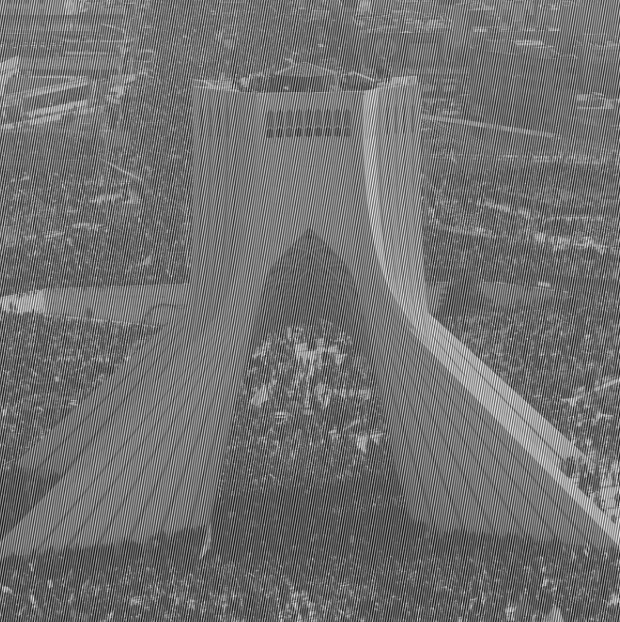
\includegraphics{wiki/compression.jpg}
\caption{uncompressed image}
\end{figure}

    \hypertarget{a}{%
\subsubsection{3.A}\label{a}}

First we obtain DCT of the image, then we use masks to zero most of
coefficient that are exists in the right corner of the DCT transform.

    \begin{Verbatim}[commandchars=\\\{\}]
{\color{incolor}In [{\color{incolor}403}]:} \PY{n}{image} \PY{o}{=} \PY{n}{cv2}\PY{o}{.}\PY{n}{imread}\PY{p}{(}\PY{l+s+s1}{\PYZsq{}}\PY{l+s+s1}{images/striping.bmp}\PY{l+s+s1}{\PYZsq{}}\PY{p}{,} \PY{n}{cv2}\PY{o}{.}\PY{n}{IMREAD\PYZus{}GRAYSCALE}\PY{p}{)}
          
          \PY{n}{dct} \PY{o}{=} \PY{n}{cv2}\PY{o}{.}\PY{n}{dct}\PY{p}{(}\PY{n}{np}\PY{o}{.}\PY{n}{float32}\PY{p}{(}\PY{n}{image}\PY{p}{)}\PY{p}{)}
          
          \PY{c+c1}{\PYZsh{} plot}
          \PY{n}{fig}\PY{p}{,} \PY{n}{ax} \PY{o}{=} \PY{n}{plt}\PY{o}{.}\PY{n}{subplots}\PY{p}{(}\PY{n}{nrows}\PY{o}{=}\PY{l+m+mi}{1}\PY{p}{,} \PY{n}{ncols}\PY{o}{=}\PY{l+m+mi}{2}\PY{p}{,} \PY{n}{figsize}\PY{o}{=}\PY{p}{(}\PY{l+m+mi}{20}\PY{p}{,} \PY{l+m+mi}{15}\PY{p}{)}\PY{p}{)}
          
          \PY{n}{ax}\PY{p}{[}\PY{l+m+mi}{0}\PY{p}{]}\PY{o}{.}\PY{n}{set\PYZus{}title}\PY{p}{(}\PY{l+s+s1}{\PYZsq{}}\PY{l+s+s1}{Original}\PY{l+s+s1}{\PYZsq{}}\PY{p}{)}
          \PY{n}{ax}\PY{p}{[}\PY{l+m+mi}{0}\PY{p}{]}\PY{o}{.}\PY{n}{imshow}\PY{p}{(}\PY{n}{image}\PY{p}{,} \PY{n}{cmap}\PY{o}{=}\PY{l+s+s1}{\PYZsq{}}\PY{l+s+s1}{gray}\PY{l+s+s1}{\PYZsq{}}\PY{p}{)}
          
          \PY{n}{ax}\PY{p}{[}\PY{l+m+mi}{1}\PY{p}{]}\PY{o}{.}\PY{n}{set\PYZus{}title}\PY{p}{(}\PY{l+s+s1}{\PYZsq{}}\PY{l+s+s1}{DCT}\PY{l+s+s1}{\PYZsq{}}\PY{p}{)}
          \PY{c+c1}{\PYZsh{} because the size of image is huge, I have just ploted the top 50x50 pixel of coefficients}
          \PY{n}{ax}\PY{p}{[}\PY{l+m+mi}{1}\PY{p}{]}\PY{o}{.}\PY{n}{imshow}\PY{p}{(}\PY{n}{dct}\PY{p}{[}\PY{p}{:}\PY{l+m+mi}{50}\PY{p}{,}\PY{l+m+mi}{0}\PY{p}{:}\PY{l+m+mi}{50}\PY{p}{]}\PY{p}{,} \PY{n}{cmap} \PY{o}{=} \PY{l+s+s1}{\PYZsq{}}\PY{l+s+s1}{gray}\PY{l+s+s1}{\PYZsq{}}\PY{p}{)}  
\end{Verbatim}


\begin{Verbatim}[commandchars=\\\{\}]
{\color{outcolor}Out[{\color{outcolor}403}]:} <matplotlib.image.AxesImage at 0x24b1d96c5f8>
\end{Verbatim}
            
    \begin{center}
    \adjustimage{max size={0.9\linewidth}{0.9\paperheight}}{output_21_1.png}
    \end{center}
    { \hspace*{\fill} \\}
    
    \begin{Verbatim}[commandchars=\\\{\}]
{\color{incolor}In [{\color{incolor}404}]:} \PY{n}{rows} \PY{o}{=} \PY{l+m+mi}{250}
          \PY{n}{columns} \PY{o}{=} \PY{l+m+mi}{250}
          \PY{n}{dct}\PY{p}{[}\PY{n}{rows}\PY{p}{:}\PY{p}{,} \PY{p}{:}\PY{p}{]} \PY{o}{=} \PY{l+m+mi}{0}  \PY{c+c1}{\PYZsh{} 50 150}
          \PY{n}{dct}\PY{p}{[}\PY{p}{:}\PY{p}{,} \PY{n}{columns}\PY{p}{:}\PY{p}{]} \PY{o}{=} \PY{l+m+mi}{0}  \PY{c+c1}{\PYZsh{} 50 150}
          \PY{n}{idct} \PY{o}{=} \PY{n}{cv2}\PY{o}{.}\PY{n}{idct}\PY{p}{(}\PY{n}{dct}\PY{p}{)}
          \PY{n}{plt}\PY{o}{.}\PY{n}{imshow}\PY{p}{(}\PY{n}{idct}\PY{p}{,} \PY{n}{cmap}\PY{o}{=}\PY{l+s+s1}{\PYZsq{}}\PY{l+s+s1}{gray}\PY{l+s+s1}{\PYZsq{}}\PY{p}{)}
          \PY{n}{cv2}\PY{o}{.}\PY{n}{imwrite}\PY{p}{(}\PY{l+s+s1}{\PYZsq{}}\PY{l+s+s1}{compressed\PYZus{}denoised.bmp}\PY{l+s+s1}{\PYZsq{}}\PY{p}{,} \PY{n}{np}\PY{o}{.}\PY{n}{uint8}\PY{p}{(}\PY{n}{idct}\PY{p}{)}\PY{p}{)}
\end{Verbatim}


\begin{Verbatim}[commandchars=\\\{\}]
{\color{outcolor}Out[{\color{outcolor}404}]:} True
\end{Verbatim}
            
    \begin{center}
    \adjustimage{max size={0.9\linewidth}{0.9\paperheight}}{output_22_1.png}
    \end{center}
    { \hspace*{\fill} \\}
    
    First step of compression is transformation and we do this using DCT
transform. This image contains a lot of vertical strips which means the
ending column of the DCT transform have high coefficients. Furthermore,
we can see many diagonal noises too so as we can see in the below image,
when we move to the right corner of DCT, coefficient are still high. The
below image is 20x20 image of the bottom-corner of the DCT transform and
in a natural image, these values almost must be zero or near but we can
see this is not happening here.

    \begin{Verbatim}[commandchars=\\\{\}]
{\color{incolor}In [{\color{incolor}405}]:} \PY{n}{plt}\PY{o}{.}\PY{n}{imshow}\PY{p}{(}\PY{n}{dct\PYZus{}temp}\PY{p}{[}\PY{o}{\PYZhy{}}\PY{l+m+mi}{20}\PY{p}{:}\PY{p}{,}\PY{o}{\PYZhy{}}\PY{l+m+mi}{20}\PY{p}{:}\PY{p}{]}\PY{p}{,} \PY{n}{cmap} \PY{o}{=} \PY{l+s+s1}{\PYZsq{}}\PY{l+s+s1}{gray}\PY{l+s+s1}{\PYZsq{}}\PY{p}{)}
\end{Verbatim}


\begin{Verbatim}[commandchars=\\\{\}]
{\color{outcolor}Out[{\color{outcolor}405}]:} <matplotlib.image.AxesImage at 0x24b1de80f60>
\end{Verbatim}
            
    \begin{center}
    \adjustimage{max size={0.9\linewidth}{0.9\paperheight}}{output_24_1.png}
    \end{center}
    { \hspace*{\fill} \\}
    
    On the other hand, we know that most of signal's energy is concentrated
on the first coefficient (top-left-corner). Here is the image of DCT
transform in 20x20 pixel:

    \begin{Verbatim}[commandchars=\\\{\}]
{\color{incolor}In [{\color{incolor}406}]:} \PY{n}{plt}\PY{o}{.}\PY{n}{imshow}\PY{p}{(}\PY{n}{dct\PYZus{}temp}\PY{p}{[}\PY{p}{:}\PY{l+m+mi}{20}\PY{p}{,}\PY{p}{:}\PY{l+m+mi}{20}\PY{p}{]}\PY{p}{,} \PY{n}{cmap} \PY{o}{=} \PY{l+s+s1}{\PYZsq{}}\PY{l+s+s1}{gray}\PY{l+s+s1}{\PYZsq{}}\PY{p}{)}
\end{Verbatim}


\begin{Verbatim}[commandchars=\\\{\}]
{\color{outcolor}Out[{\color{outcolor}406}]:} <matplotlib.image.AxesImage at 0x24b1ded2f28>
\end{Verbatim}
            
    \begin{center}
    \adjustimage{max size={0.9\linewidth}{0.9\paperheight}}{output_26_1.png}
    \end{center}
    { \hspace*{\fill} \\}
    
    So the idea is here to zero all those coefficients which correspond to
the noises and we do this by this line of code:

\begin{Shaded}
\begin{Highlighting}[]
\NormalTok{dct[}\DecValTok{250}\NormalTok{:, }\DecValTok{250}\NormalTok{:] }\OperatorTok{=} \DecValTok{0} 
\end{Highlighting}
\end{Shaded}

Now we have reduced information which most of them were noises and we
just need to say how many zeros we have in term of length. Example:

\begin{verbatim}
[1, 2, 3, 0, 0, 0, 0, 0, 0, 0, 0, 0, 0] -> [1, 2, 3,, 1, 3, 13, 1] 
\end{verbatim}

4 last values represent shape of compressed image and final image
respectively. so we can obtain number of zeros just by it.

    \begin{Verbatim}[commandchars=\\\{\}]
{\color{incolor}In [{\color{incolor}407}]:} \PY{k}{def} \PY{n+nf}{compress}\PY{p}{(}\PY{n}{dct}\PY{p}{,} \PY{n}{rows}\PY{p}{,} \PY{n}{columns}\PY{p}{,} \PY{n}{save}\PY{o}{=}\PY{k+kc}{True}\PY{p}{)}\PY{p}{:}
              \PY{l+s+sd}{\PYZdq{}\PYZdq{}\PYZdq{}}
          \PY{l+s+sd}{    Compresses image using given DCT coefficient values and number of non\PYZhy{}zero rows and columns}
          \PY{l+s+sd}{    }
          \PY{l+s+sd}{    :param dct: }
          \PY{l+s+sd}{    :param rows:}
          \PY{l+s+sd}{    :param columns:}
          \PY{l+s+sd}{    :param save:}
          \PY{l+s+sd}{    :return:}
          \PY{l+s+sd}{    \PYZdq{}\PYZdq{}\PYZdq{}}
              \PY{n}{shape} \PY{o}{=} \PY{n}{dct}\PY{o}{.}\PY{n}{shape}
              \PY{n}{shapes} \PY{o}{=} \PY{n}{np}\PY{o}{.}\PY{n}{array}\PY{p}{(}\PY{p}{[}\PY{n}{rows}\PY{p}{,} \PY{n}{columns}\PY{p}{,} \PY{n}{dct}\PY{o}{.}\PY{n}{shape}\PY{p}{[}\PY{l+m+mi}{0}\PY{p}{]}\PY{p}{,} \PY{n}{dct}\PY{o}{.}\PY{n}{shape}\PY{p}{[}\PY{l+m+mi}{1}\PY{p}{]}\PY{p}{]}\PY{p}{)}
              \PY{n}{compressed} \PY{o}{=} \PY{n}{np}\PY{o}{.}\PY{n}{empty}\PY{p}{(}\PY{n}{rows}\PY{o}{*}\PY{n}{columns}\PY{o}{+}\PY{l+m+mi}{4}\PY{p}{)}
              \PY{n}{compressed}\PY{p}{[}\PY{p}{:}\PY{n}{rows}\PY{o}{*}\PY{n}{columns}\PY{p}{]} \PY{o}{=} \PY{n}{dct}\PY{p}{[}\PY{p}{:}\PY{n}{rows}\PY{p}{,} \PY{p}{:}\PY{n}{columns}\PY{p}{]}\PY{o}{.}\PY{n}{flatten}\PY{p}{(}\PY{p}{)}
              \PY{k}{for} \PY{n}{idx}\PY{p}{,} \PY{n}{s} \PY{o+ow}{in} \PY{n+nb}{zip}\PY{p}{(}\PY{p}{[}\PY{o}{\PYZhy{}}\PY{l+m+mi}{4}\PY{p}{,}\PY{o}{\PYZhy{}}\PY{l+m+mi}{3}\PY{p}{,}\PY{o}{\PYZhy{}}\PY{l+m+mi}{2}\PY{p}{,}\PY{o}{\PYZhy{}}\PY{l+m+mi}{1}\PY{p}{]}\PY{p}{,} \PY{n}{shapes}\PY{p}{)}\PY{p}{:}
                  \PY{n}{compressed}\PY{p}{[}\PY{n}{idx}\PY{p}{]} \PY{o}{=} \PY{n}{s}
              \PY{k}{if} \PY{n}{save}\PY{p}{:}
                  \PY{n}{np}\PY{o}{.}\PY{n}{save}\PY{p}{(}\PY{l+s+s1}{\PYZsq{}}\PY{l+s+s1}{compressed\PYZus{}denoised\PYZus{}data.npy}\PY{l+s+s1}{\PYZsq{}}\PY{p}{,} \PY{n}{compressed}\PY{p}{,} \PY{k+kc}{False}\PY{p}{,} \PY{k+kc}{False}\PY{p}{)}
              \PY{k}{return} \PY{n}{compressed}
          \PY{n}{compressed\PYZus{}image} \PY{o}{=} \PY{n}{compress}\PY{p}{(}\PY{n}{dct}\PY{p}{,} \PY{n}{rows}\PY{p}{,} \PY{n}{columns}\PY{p}{)}
          \PY{n+nb}{print}\PY{p}{(}\PY{l+s+s1}{\PYZsq{}}\PY{l+s+s1}{Compression ratio: }\PY{l+s+si}{\PYZob{}\PYZcb{}}\PY{l+s+s1}{\PYZsq{}}\PY{o}{.}\PY{n}{format}\PY{p}{(}\PY{n}{compressed}\PY{o}{.}\PY{n}{shape}\PY{p}{[}\PY{l+m+mi}{0}\PY{p}{]}\PY{o}{*}\PY{l+m+mi}{100}\PY{o}{/}\PY{p}{(}\PY{n}{dct}\PY{o}{.}\PY{n}{shape}\PY{p}{[}\PY{l+m+mi}{0}\PY{p}{]}\PY{o}{*}\PY{n}{dct}\PY{o}{.}\PY{n}{shape}\PY{p}{[}\PY{l+m+mi}{1}\PY{p}{]}\PY{p}{)}\PY{p}{)}\PY{p}{)}
\end{Verbatim}


    \begin{Verbatim}[commandchars=\\\{\}]
Compression ratio: 0.42517700599236674

    \end{Verbatim}

    In this section now we do reverse what we have done in \texttt{compress}
method to get uncompressed numpy array.

    \begin{Verbatim}[commandchars=\\\{\}]
{\color{incolor}In [{\color{incolor}429}]:} \PY{k}{def} \PY{n+nf}{uncompress}\PY{p}{(}\PY{n}{path}\PY{p}{)}\PY{p}{:}
              \PY{l+s+sd}{\PYZdq{}\PYZdq{}\PYZdq{}}
          \PY{l+s+sd}{    Gets a path to .npy file containing compressed image and decompress it to a standard DCT array.}
          \PY{l+s+sd}{    }
          \PY{l+s+sd}{    :param path: path to a .npy file in specified format}
          \PY{l+s+sd}{    :return: a numpy ndarray}
          \PY{l+s+sd}{    \PYZdq{}\PYZdq{}\PYZdq{}}
              \PY{n}{compressed\PYZus{}image} \PY{o}{=} \PY{n}{np}\PY{o}{.}\PY{n}{load}\PY{p}{(}\PY{n}{path}\PY{p}{)}
              \PY{n}{shape} \PY{o}{=} \PY{p}{(}\PY{n}{np}\PY{o}{.}\PY{n}{int}\PY{p}{(}\PY{n}{compressed\PYZus{}image}\PY{p}{[}\PY{o}{\PYZhy{}}\PY{l+m+mi}{2}\PY{p}{]}\PY{p}{)}\PY{p}{,} \PY{n}{np}\PY{o}{.}\PY{n}{int}\PY{p}{(}\PY{n}{compressed\PYZus{}image}\PY{p}{[}\PY{o}{\PYZhy{}}\PY{l+m+mi}{1}\PY{p}{]}\PY{p}{)}\PY{p}{)}
              \PY{n}{rows} \PY{o}{=} \PY{n}{np}\PY{o}{.}\PY{n}{int}\PY{p}{(}\PY{n}{compressed\PYZus{}image}\PY{p}{[}\PY{o}{\PYZhy{}}\PY{l+m+mi}{4}\PY{p}{]}\PY{p}{)}
              \PY{n}{columns} \PY{o}{=} \PY{n}{np}\PY{o}{.}\PY{n}{int}\PY{p}{(}\PY{n}{compressed\PYZus{}image}\PY{p}{[}\PY{o}{\PYZhy{}}\PY{l+m+mi}{3}\PY{p}{]}\PY{p}{)}
              \PY{n}{uncompressed\PYZus{}image} \PY{o}{=} \PY{n}{np}\PY{o}{.}\PY{n}{zeros}\PY{p}{(}\PY{n}{shape}\PY{p}{)}
              \PY{n}{uncompressed\PYZus{}image}\PY{p}{[}\PY{p}{:}\PY{n}{rows}\PY{p}{,} \PY{p}{:}\PY{n}{columns}\PY{p}{]} \PY{o}{=} \PY{n}{compressed\PYZus{}image}\PY{p}{[}\PY{p}{:}\PY{o}{\PYZhy{}}\PY{l+m+mi}{4}\PY{p}{]}\PY{o}{.}\PY{n}{reshape}\PY{p}{(}\PY{n}{rows}\PY{p}{,} \PY{n}{columns}\PY{p}{)}
              \PY{n}{uncompressed\PYZus{}image} \PY{o}{=} \PY{n}{uncompressed\PYZus{}image}\PY{o}{.}\PY{n}{astype}\PY{p}{(}\PY{n}{np}\PY{o}{.}\PY{n}{float32}\PY{p}{)}
              \PY{k}{return} \PY{n}{uncompressed\PYZus{}image}
          
          \PY{n}{uncompressed\PYZus{}image}\PY{o}{=} \PY{n}{uncompress}\PY{p}{(}\PY{l+s+s1}{\PYZsq{}}\PY{l+s+s1}{compressed\PYZus{}denoised\PYZus{}data.npy}\PY{l+s+s1}{\PYZsq{}}\PY{p}{)}
\end{Verbatim}


    The last step will be inverse-DCT to get image and \texttt{cv2.idct()}
is able to do this.

    \begin{Verbatim}[commandchars=\\\{\}]
{\color{incolor}In [{\color{incolor}430}]:} \PY{n}{idct} \PY{o}{=} \PY{n}{cv2}\PY{o}{.}\PY{n}{idct}\PY{p}{(}\PY{n}{uncompressed\PYZus{}image}\PY{p}{)}
          \PY{n}{plt}\PY{o}{.}\PY{n}{imshow}\PY{p}{(}\PY{n}{idct}\PY{p}{,} \PY{n}{cmap}\PY{o}{=}\PY{l+s+s1}{\PYZsq{}}\PY{l+s+s1}{gray}\PY{l+s+s1}{\PYZsq{}}\PY{p}{)}
\end{Verbatim}


\begin{Verbatim}[commandchars=\\\{\}]
{\color{outcolor}Out[{\color{outcolor}430}]:} <matplotlib.image.AxesImage at 0x24b1de35d30>
\end{Verbatim}
            
    \begin{center}
    \adjustimage{max size={0.9\linewidth}{0.9\paperheight}}{output_32_1.png}
    \end{center}
    { \hspace*{\fill} \\}
    
    \hypertarget{create-2d-dct-from-1d-based-on-separable-kernels}{%
\subsection{4 Create 2D DCT From 1D Based on Separable
Kernels}\label{create-2d-dct-from-1d-based-on-separable-kernels}}

\begin{enumerate}
\def\labelenumi{\arabic{enumi}.}
\tightlist
\item
  Show the mathematical calculations to obtain the 2D \texttt{DCT}.
\item
  Write a program to calculate \texttt{DCT} of an image using your
  approach.
\item
  Apply your \texttt{DCT} function from step 2 on \texttt{image1.tif}
  and compare your result the one obtained from question 2.
\end{enumerate}

    \hypertarget{a-mathematical-calculations}{%
\subsubsection{4.A Mathematical
Calculations}\label{a-mathematical-calculations}}

    \begin{figure}
\centering
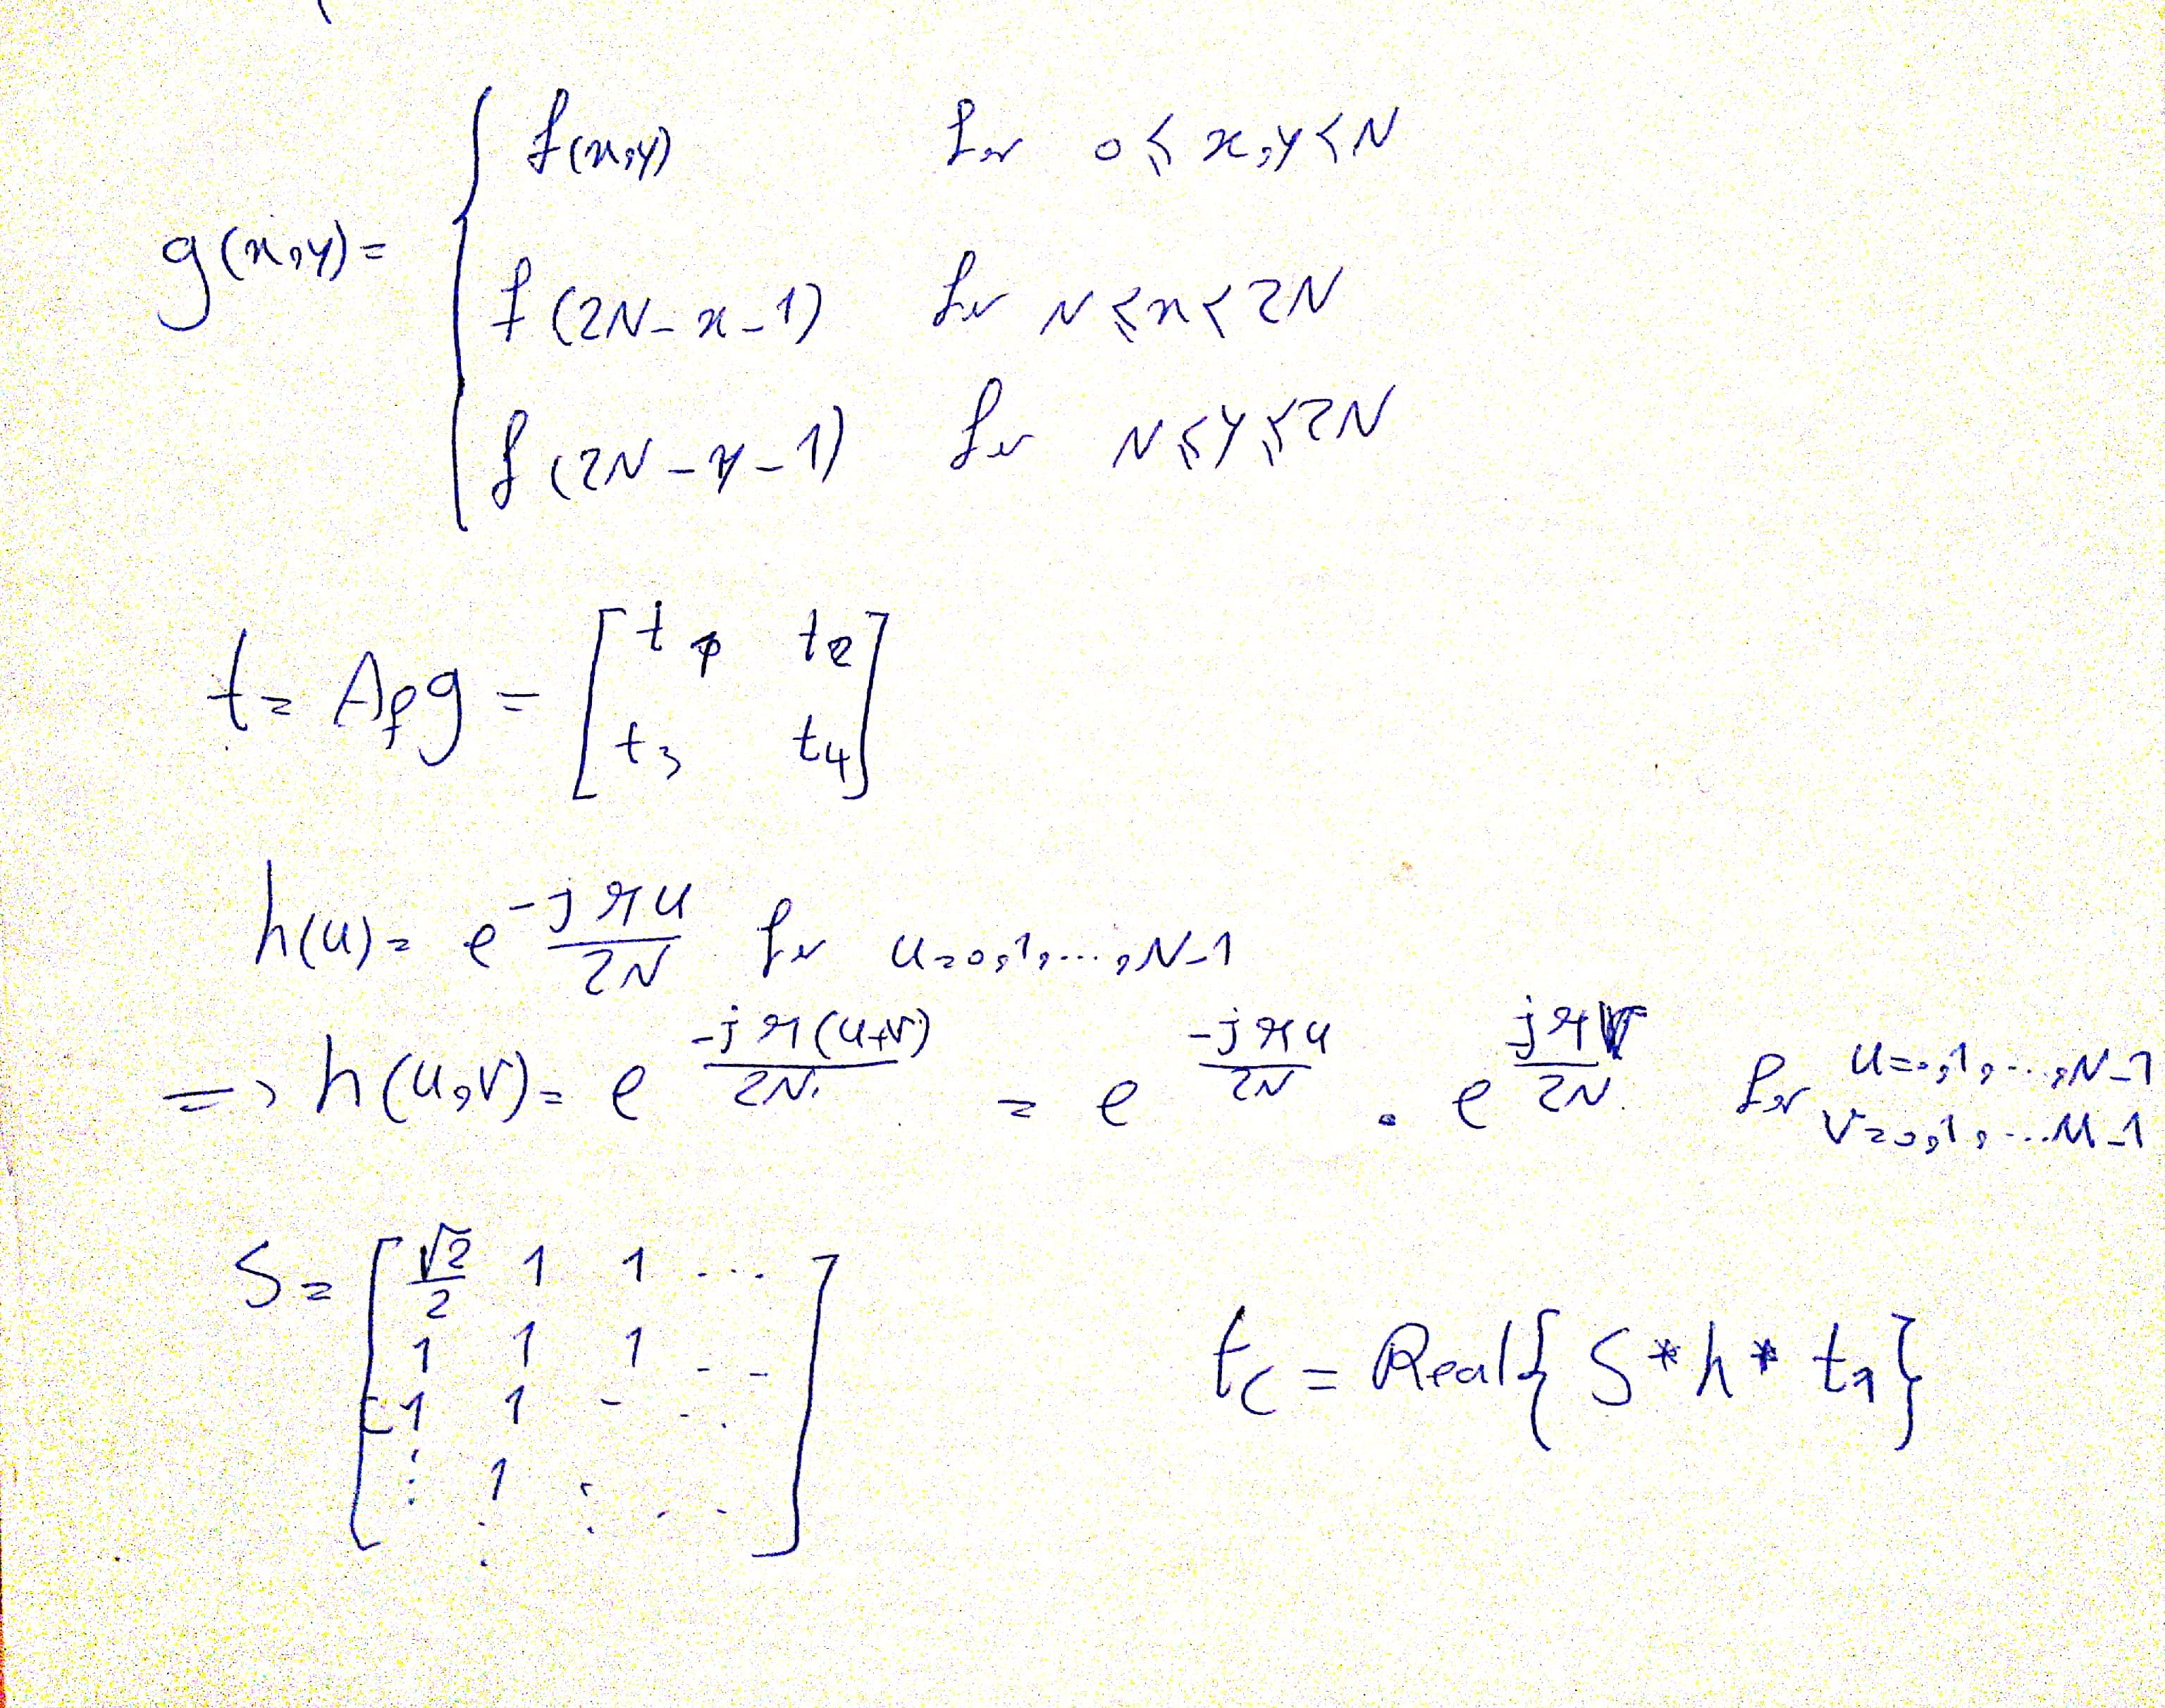
\includegraphics{wiki/dct_fft.jpg}
\caption{2d DCT mathematics using FFT}
\end{figure}

    I MISUNDERSTOOD THE QUESTION AND IMPLEMENTED 2D DCT USING 1D DCT TOO.

\begin{figure}
\centering
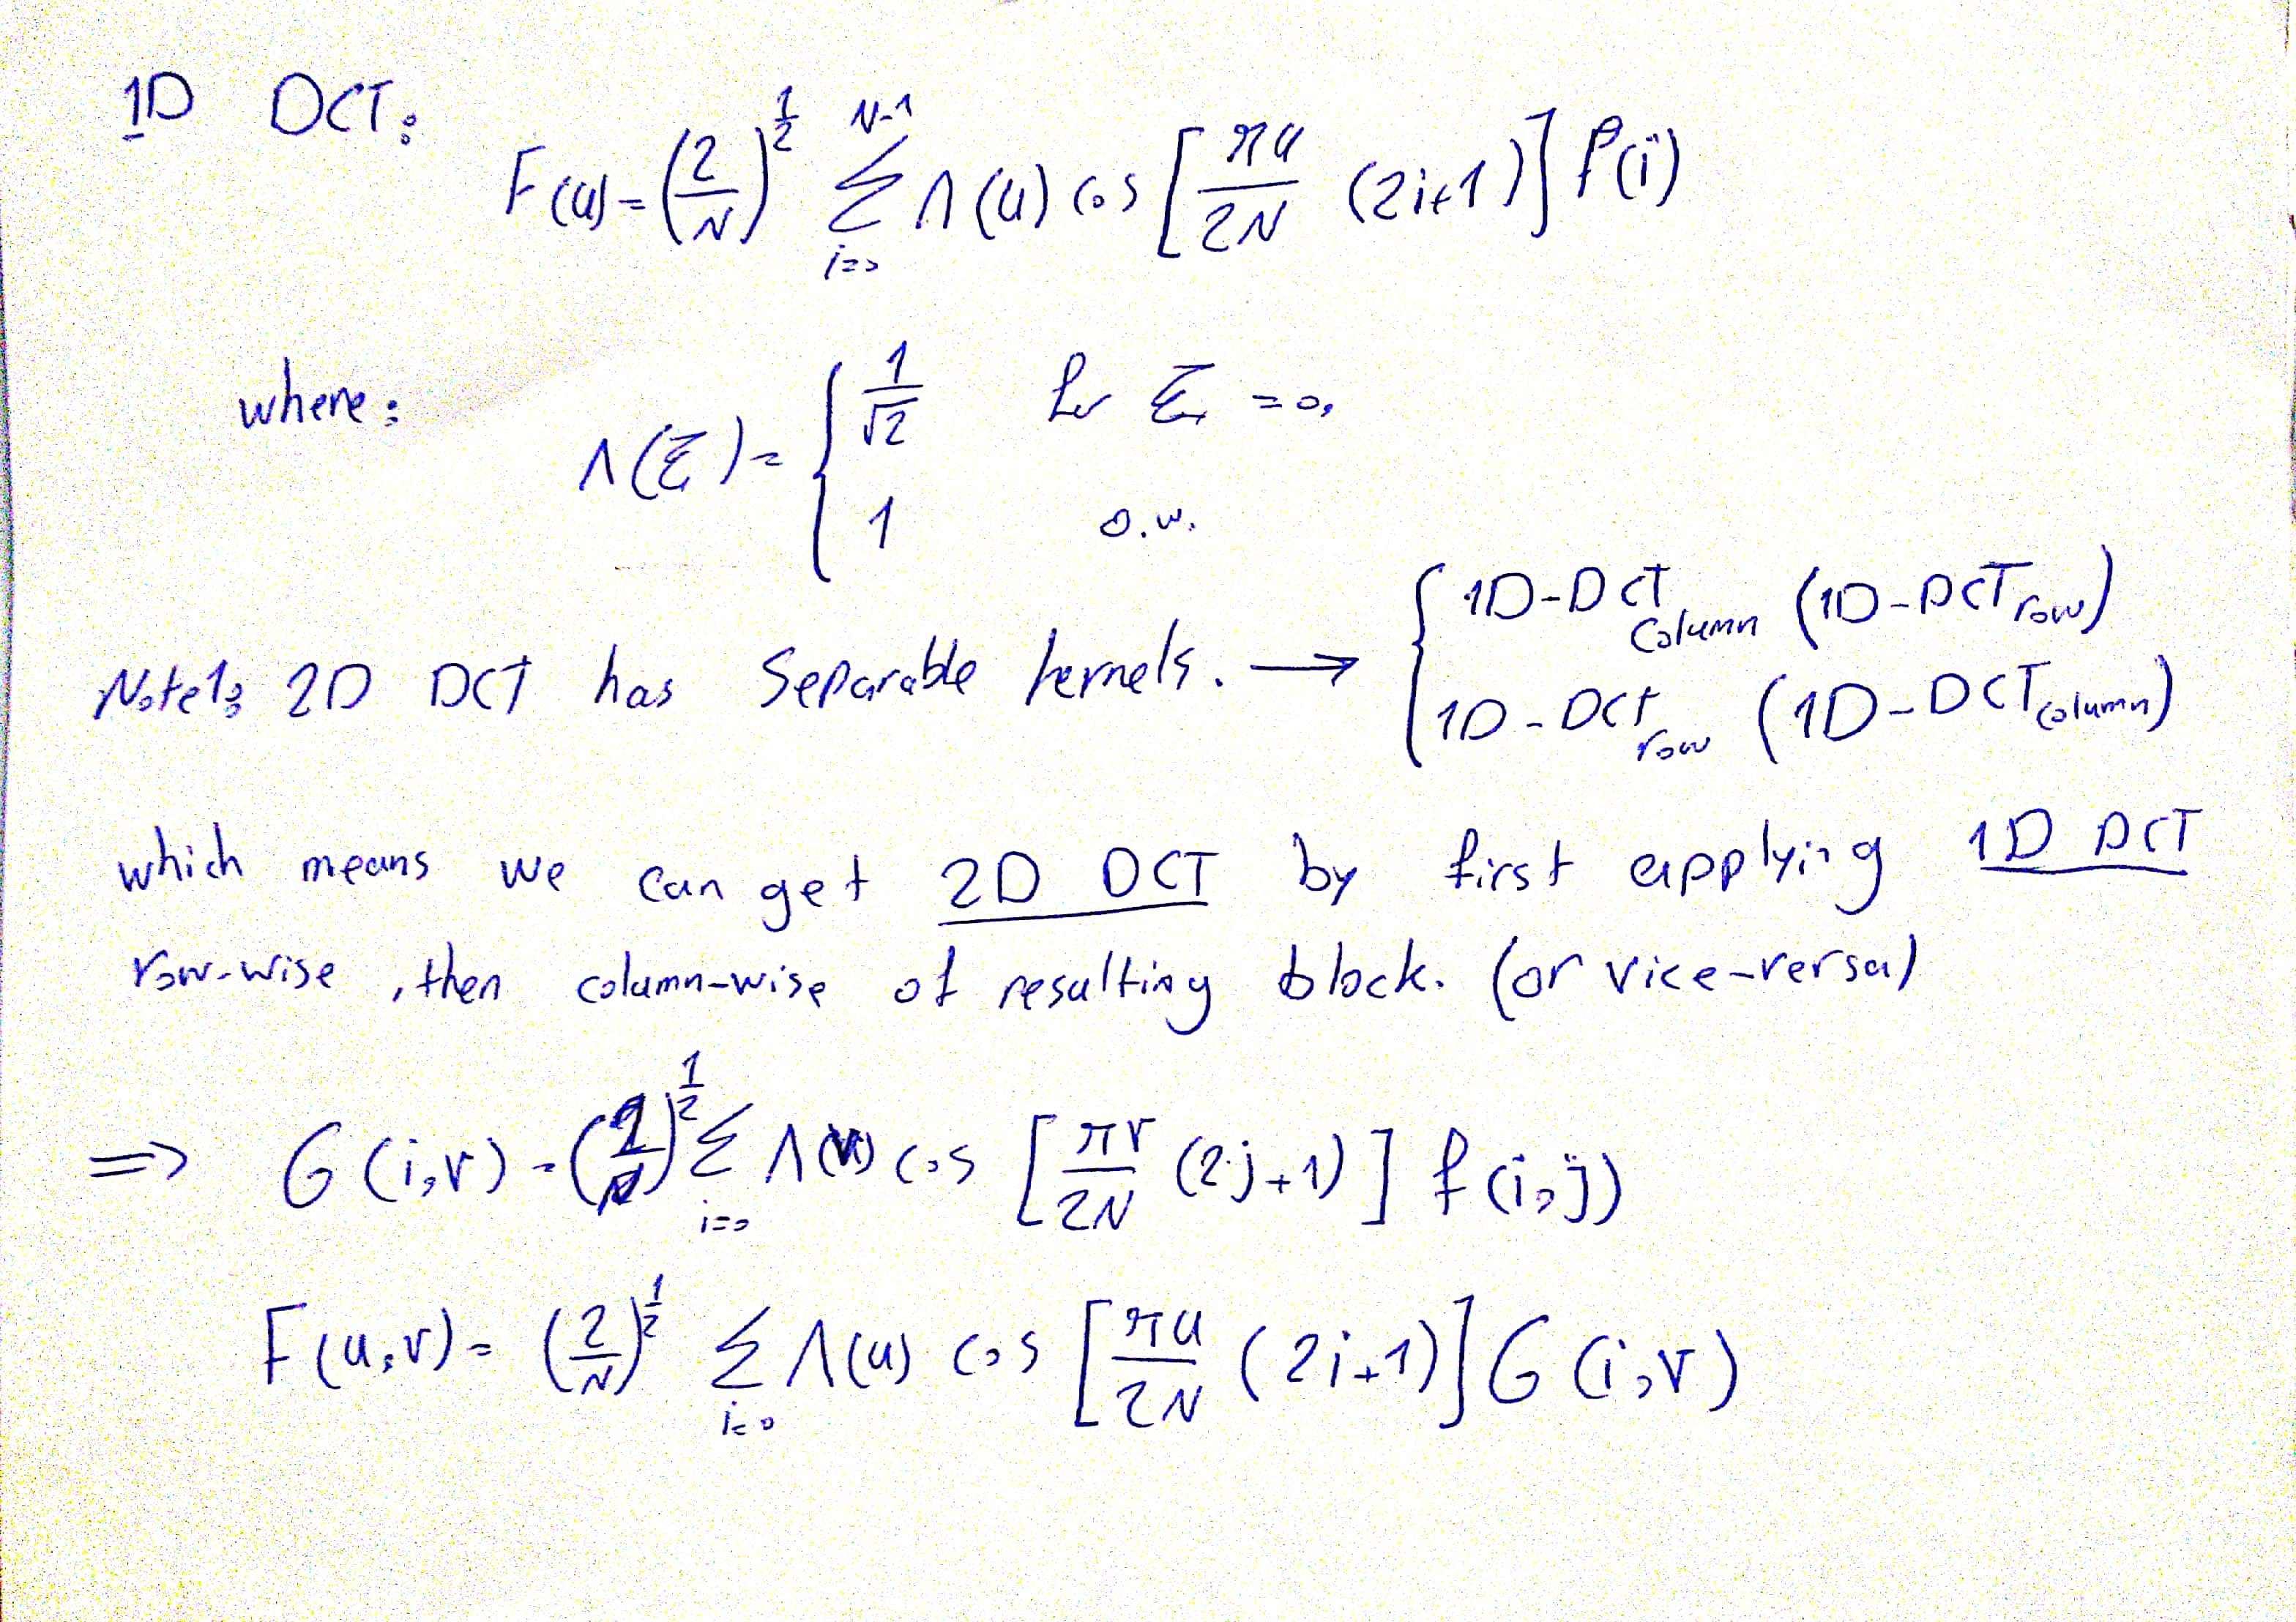
\includegraphics{wiki/4.1.jpg}
\caption{2d DCT mathematics using 1D DCT}
\end{figure}

    \hypertarget{b-implementation}{%
\subsubsection{4.B Implementation}\label{b-implementation}}

    \begin{Verbatim}[commandchars=\\\{\}]
{\color{incolor}In [{\color{incolor}113}]:} \PY{k}{def} \PY{n+nf}{dct\PYZus{}from\PYZus{}fft}\PY{p}{(}\PY{n}{signal}\PY{p}{)}\PY{p}{:}
              \PY{l+s+sd}{\PYZdq{}\PYZdq{}\PYZdq{}}
          \PY{l+s+sd}{    Calculates 2D DCT from 1D FFT (Page 489 and 490 of Gonzales 4th ed.)}
          \PY{l+s+sd}{    }
          \PY{l+s+sd}{    :param signal: input spatial signal in form of numpy ndarray}
          \PY{l+s+sd}{    :return: 2D DCT of input in form of numpy ndarray}
          \PY{l+s+sd}{    \PYZdq{}\PYZdq{}\PYZdq{}}
              \PY{n}{r}\PY{p}{,}\PY{n}{c} \PY{o}{=} \PY{n}{signal}\PY{o}{.}\PY{n}{shape}
              \PY{n}{g} \PY{o}{=} \PY{n}{np}\PY{o}{.}\PY{n}{zeros}\PY{p}{(}\PY{p}{(}\PY{n}{r}\PY{o}{*}\PY{l+m+mi}{2}\PY{p}{,} \PY{n}{c}\PY{o}{*}\PY{l+m+mi}{2}\PY{p}{)}\PY{p}{)}
              \PY{n}{g}\PY{p}{[}\PY{p}{:}\PY{n}{r}\PY{p}{,} \PY{p}{:}\PY{n}{c}\PY{p}{]} \PY{o}{=} \PY{n}{signal}
              \PY{n}{g}\PY{p}{[}\PY{p}{:}\PY{n}{r}\PY{p}{,}\PY{n}{c}\PY{p}{:}\PY{p}{]} \PY{o}{=} \PY{n}{np}\PY{o}{.}\PY{n}{flip}\PY{p}{(}\PY{n}{signal}\PY{p}{,} \PY{n}{axis}\PY{o}{=}\PY{l+m+mi}{1}\PY{p}{)}
              \PY{n}{g}\PY{p}{[}\PY{n}{r}\PY{p}{:}\PY{p}{,}\PY{p}{:}\PY{p}{]} \PY{o}{=} \PY{n}{np}\PY{o}{.}\PY{n}{flip}\PY{p}{(}\PY{n}{g}\PY{p}{[}\PY{p}{:}\PY{n}{r}\PY{p}{,}\PY{p}{:}\PY{p}{]}\PY{p}{,} \PY{n}{axis}\PY{o}{=}\PY{l+m+mi}{0}\PY{p}{)}
              \PY{n}{ft} \PY{o}{=} \PY{n}{np}\PY{o}{.}\PY{n}{fft}\PY{o}{.}\PY{n}{fft2}\PY{p}{(}\PY{n}{g}\PY{p}{)}\PY{p}{[}\PY{p}{:}\PY{n}{r}\PY{p}{,}\PY{p}{:}\PY{n}{c}\PY{p}{]}
              \PY{n}{h} \PY{o}{=} \PY{n}{np}\PY{o}{.}\PY{n}{zeros}\PY{p}{(}\PY{n}{signal}\PY{o}{.}\PY{n}{shape}\PY{p}{,} \PY{n}{dtype}\PY{o}{=}\PY{n+nb}{complex}\PY{p}{)}
              \PY{k}{for} \PY{n}{i} \PY{o+ow}{in} \PY{n+nb}{range}\PY{p}{(}\PY{n}{signal}\PY{o}{.}\PY{n}{shape}\PY{p}{[}\PY{l+m+mi}{0}\PY{p}{]}\PY{p}{)}\PY{p}{:}
                  \PY{k}{for} \PY{n}{j} \PY{o+ow}{in} \PY{n+nb}{range}\PY{p}{(}\PY{n}{signal}\PY{o}{.}\PY{n}{shape}\PY{p}{[}\PY{l+m+mi}{1}\PY{p}{]}\PY{p}{)}\PY{p}{:}
                      \PY{n}{h}\PY{p}{[}\PY{n}{i}\PY{p}{,}\PY{n}{j}\PY{p}{]} \PY{o}{=} \PY{n}{np}\PY{o}{.}\PY{n}{exp}\PY{p}{(}\PY{o}{\PYZhy{}}\PY{l+m+mi}{1}\PY{n}{j}\PY{o}{*}\PY{n}{np}\PY{o}{.}\PY{n}{pi}\PY{o}{*}\PY{n}{j}\PY{o}{/}\PY{p}{(}\PY{l+m+mi}{2}\PY{o}{*}\PY{n}{signal}\PY{o}{.}\PY{n}{shape}\PY{p}{[}\PY{l+m+mi}{1}\PY{p}{]}\PY{p}{)}\PY{p}{)} \PY{o}{*} \PY{n}{np}\PY{o}{.}\PY{n}{exp}\PY{p}{(}\PY{o}{\PYZhy{}}\PY{l+m+mi}{1}\PY{n}{j}\PY{o}{*}\PY{n}{np}\PY{o}{.}\PY{n}{pi}\PY{o}{*}\PY{n}{i}\PY{o}{/}\PY{p}{(}\PY{l+m+mi}{2}\PY{o}{*}\PY{n}{signal}\PY{o}{.}\PY{n}{shape}\PY{p}{[}\PY{l+m+mi}{0}\PY{p}{]}\PY{p}{)}\PY{p}{)}
              \PY{n}{s} \PY{o}{=} \PY{n}{np}\PY{o}{.}\PY{n}{ones}\PY{p}{(}\PY{n}{signal}\PY{o}{.}\PY{n}{shape}\PY{p}{)}
              \PY{n}{s}\PY{p}{[}\PY{l+m+mi}{0}\PY{p}{,}\PY{l+m+mi}{0}\PY{p}{]} \PY{o}{=} \PY{l+m+mf}{1.}\PY{o}{/}\PY{n}{np}\PY{o}{.}\PY{n}{sqrt}\PY{p}{(}\PY{l+m+mi}{2}\PY{p}{)}
              \PY{n}{dct} \PY{o}{=} \PY{n}{np}\PY{o}{.}\PY{n}{real}\PY{p}{(}\PY{n}{s}\PY{o}{*}\PY{n}{h}\PY{o}{*}\PY{n}{ft}\PY{p}{)}\PY{o}{/}\PY{p}{(}\PY{n}{np}\PY{o}{.}\PY{n}{sqrt}\PY{p}{(}\PY{l+m+mi}{2}\PY{o}{*}\PY{n}{r}\PY{o}{*}\PY{n}{r}\PY{o}{*}\PY{n}{c}\PY{o}{*}\PY{n}{c}\PY{p}{)}\PY{p}{)}
              \PY{k}{return} \PY{n}{dct} 
\end{Verbatim}


    \begin{Verbatim}[commandchars=\\\{\}]
{\color{incolor}In [{\color{incolor}54}]:} \PY{c+c1}{\PYZsh{}\PYZsh{} I MISUNDERSTOOD THE QUESTION AND IMPLEMENTED 2D DCT USING 1D DCT TOO.}
         
         \PY{k}{def} \PY{n+nf}{dct}\PY{p}{(}\PY{n}{signal}\PY{p}{,} \PY{n}{dim}\PY{o}{=}\PY{l+m+mi}{2}\PY{p}{)}\PY{p}{:}
             \PY{l+s+sd}{\PYZdq{}\PYZdq{}\PYZdq{}}
         \PY{l+s+sd}{    }
         \PY{l+s+sd}{    :param signal: Input spatial domain signal (numpy ndarray)}
         \PY{l+s+sd}{    :param dim: Whether use 2D DCT or 1D DCT}
         \PY{l+s+sd}{    :return: DCT coefficients of signal (numpy ndarray)}
         \PY{l+s+sd}{    \PYZdq{}\PYZdq{}\PYZdq{}}
             \PY{c+c1}{\PYZsh{} horizontal}
             \PY{n}{g} \PY{o}{=} \PY{n}{np}\PY{o}{.}\PY{n}{zeros}\PY{p}{(}\PY{n}{signal}\PY{o}{.}\PY{n}{shape}\PY{p}{)}
             \PY{n}{c} \PY{o}{=} \PY{l+m+mi}{0}
             \PY{k}{for} \PY{n}{v} \PY{o+ow}{in} \PY{n+nb}{range}\PY{p}{(}\PY{n}{signal}\PY{o}{.}\PY{n}{shape}\PY{p}{[}\PY{l+m+mi}{0}\PY{p}{]}\PY{p}{)}\PY{p}{:}
                 \PY{k}{for} \PY{n}{j} \PY{o+ow}{in} \PY{n+nb}{range}\PY{p}{(}\PY{n}{signal}\PY{o}{.}\PY{n}{shape}\PY{p}{[}\PY{l+m+mi}{0}\PY{p}{]}\PY{p}{)}\PY{p}{:}
                     \PY{n}{c} \PY{o}{+}\PY{o}{=} \PY{n}{signal}\PY{p}{[}\PY{n}{j}\PY{p}{]}\PY{o}{*}\PY{n}{np}\PY{o}{.}\PY{n}{cos}\PY{p}{(}\PY{p}{(}\PY{l+m+mi}{2}\PY{o}{*}\PY{n}{j}\PY{o}{+}\PY{l+m+mi}{1}\PY{p}{)}\PY{o}{*}\PY{n}{np}\PY{o}{.}\PY{n}{pi}\PY{o}{*}\PY{n}{v}\PY{o}{/}\PY{p}{(}\PY{l+m+mi}{2}\PY{o}{*}\PY{n}{signal}\PY{o}{.}\PY{n}{shape}\PY{p}{[}\PY{l+m+mi}{0}\PY{p}{]}\PY{p}{)}\PY{p}{)}
                 \PY{k}{if} \PY{n}{v} \PY{o}{==} \PY{l+m+mi}{0}\PY{p}{:}
                     \PY{n}{g}\PY{p}{[}\PY{n}{v}\PY{p}{]} \PY{o}{=} \PY{n}{c}\PY{o}{*}\PY{n}{np}\PY{o}{.}\PY{n}{sqrt}\PY{p}{(}\PY{l+m+mi}{2}\PY{p}{)}\PY{o}{/}\PY{l+m+mi}{2}
                 \PY{k}{else}\PY{p}{:}
                     \PY{n}{g}\PY{p}{[}\PY{n}{v}\PY{p}{]} \PY{o}{=} \PY{n}{c}
                 \PY{n}{c}\PY{o}{=}\PY{l+m+mi}{0}
             \PY{n}{g} \PY{o}{=} \PY{n}{g}\PY{o}{*}\PY{n}{np}\PY{o}{.}\PY{n}{sqrt}\PY{p}{(}\PY{l+m+mi}{2}\PY{o}{/}\PY{n}{signal}\PY{o}{.}\PY{n}{shape}\PY{p}{[}\PY{l+m+mi}{0}\PY{p}{]}\PY{p}{)}
             \PY{k}{if} \PY{n}{dim} \PY{o}{==} \PY{l+m+mi}{1}\PY{p}{:}
                 \PY{k}{return} \PY{n}{g}
             
             \PY{c+c1}{\PYZsh{} vertical}
             \PY{n}{f} \PY{o}{=} \PY{n}{np}\PY{o}{.}\PY{n}{zeros}\PY{p}{(}\PY{n}{signal}\PY{o}{.}\PY{n}{shape}\PY{p}{)}
             \PY{n}{c} \PY{o}{=} \PY{l+m+mi}{0}
             \PY{k}{for} \PY{n}{v} \PY{o+ow}{in} \PY{n+nb}{range}\PY{p}{(}\PY{n}{g}\PY{o}{.}\PY{n}{shape}\PY{p}{[}\PY{l+m+mi}{1}\PY{p}{]}\PY{p}{)}\PY{p}{:}
                 \PY{k}{for} \PY{n}{j} \PY{o+ow}{in} \PY{n+nb}{range}\PY{p}{(}\PY{n}{g}\PY{o}{.}\PY{n}{shape}\PY{p}{[}\PY{l+m+mi}{1}\PY{p}{]}\PY{p}{)}\PY{p}{:}
                     \PY{n}{c} \PY{o}{+}\PY{o}{=} \PY{n}{g}\PY{p}{[}\PY{p}{:}\PY{p}{,}\PY{n}{j}\PY{p}{]}\PY{o}{*}\PY{n}{np}\PY{o}{.}\PY{n}{cos}\PY{p}{(}\PY{p}{(}\PY{l+m+mi}{2}\PY{o}{*}\PY{n}{j}\PY{o}{+}\PY{l+m+mi}{1}\PY{p}{)}\PY{o}{*}\PY{n}{np}\PY{o}{.}\PY{n}{pi}\PY{o}{*}\PY{n}{v}\PY{o}{/}\PY{p}{(}\PY{l+m+mi}{2}\PY{o}{*}\PY{n}{g}\PY{o}{.}\PY{n}{shape}\PY{p}{[}\PY{l+m+mi}{1}\PY{p}{]}\PY{p}{)}\PY{p}{)}
                 \PY{k}{if} \PY{n}{v} \PY{o}{==} \PY{l+m+mi}{0}\PY{p}{:}
                     \PY{n}{f}\PY{p}{[}\PY{p}{:}\PY{p}{,}\PY{n}{v}\PY{p}{]} \PY{o}{=} \PY{n}{c}\PY{o}{*}\PY{n}{np}\PY{o}{.}\PY{n}{sqrt}\PY{p}{(}\PY{l+m+mi}{2}\PY{p}{)}\PY{o}{/}\PY{l+m+mi}{2}
                 \PY{k}{else}\PY{p}{:}
                     \PY{n}{f}\PY{p}{[}\PY{p}{:}\PY{p}{,}\PY{n}{v}\PY{p}{]} \PY{o}{=} \PY{n}{c}
                 \PY{n}{c}\PY{o}{=}\PY{l+m+mi}{0}
             \PY{n}{f} \PY{o}{=} \PY{n}{f}\PY{o}{*}\PY{n}{np}\PY{o}{.}\PY{n}{sqrt}\PY{p}{(}\PY{l+m+mi}{2}\PY{o}{/}\PY{n}{g}\PY{o}{.}\PY{n}{shape}\PY{p}{[}\PY{l+m+mi}{1}\PY{p}{]}\PY{p}{)}
             \PY{k}{return} \PY{n}{f}
\end{Verbatim}


    \hypertarget{c-compare-your-dct-with-cv2.dct}{%
\subsubsection{\texorpdfstring{4.C Compare Your DCT with
\texttt{cv2.dct}}{4.C Compare Your DCT with cv2.dct}}\label{c-compare-your-dct-with-cv2.dct}}

    \begin{Verbatim}[commandchars=\\\{\}]
{\color{incolor}In [{\color{incolor}120}]:} \PY{k+kn}{import} \PY{n+nn}{time}
          \PY{n}{src\PYZus{}name} \PY{o}{=} \PY{l+s+s1}{\PYZsq{}}\PY{l+s+s1}{images/image1.tif}\PY{l+s+s1}{\PYZsq{}}
          \PY{n}{dst\PYZus{}path} \PY{o}{=} \PY{l+s+s1}{\PYZsq{}}\PY{l+s+s1}{transformed/}\PY{l+s+s1}{\PYZsq{}}
          
          \PY{n}{fig}\PY{p}{,} \PY{n}{ax} \PY{o}{=} \PY{n}{plt}\PY{o}{.}\PY{n}{subplots}\PY{p}{(}\PY{n}{nrows}\PY{o}{=}\PY{l+m+mi}{1}\PY{p}{,} \PY{n}{ncols}\PY{o}{=}\PY{l+m+mi}{3}\PY{p}{,} \PY{n}{figsize}\PY{o}{=}\PY{p}{(}\PY{l+m+mi}{20}\PY{p}{,} \PY{l+m+mi}{15}\PY{p}{)}\PY{p}{)}
          \PY{c+c1}{\PYZsh{} load image}
          \PY{n}{image} \PY{o}{=} \PY{n}{cv2}\PY{o}{.}\PY{n}{imread}\PY{p}{(}\PY{n}{src\PYZus{}name}\PY{p}{,} \PY{n}{cv2}\PY{o}{.}\PY{n}{IMREAD\PYZus{}GRAYSCALE}\PY{p}{)}
          
          \PY{c+c1}{\PYZsh{} Custom DCT}
          \PY{n}{t1} \PY{o}{=} \PY{n}{time}\PY{o}{.}\PY{n}{time}\PY{p}{(}\PY{p}{)}
          \PY{n}{custom\PYZus{}dct} \PY{o}{=} \PY{n}{dct\PYZus{}from\PYZus{}fft}\PY{p}{(}\PY{n}{image}\PY{p}{)}
          \PY{n}{t1} \PY{o}{=} \PY{n}{time}\PY{o}{.}\PY{n}{time}\PY{p}{(}\PY{p}{)}\PY{o}{\PYZhy{}} \PY{n}{t1}
          \PY{n}{custom\PYZus{}dct} \PY{o}{=} \PY{n}{custom\PYZus{}dct}\PY{o}{*}\PY{l+m+mi}{255}\PY{o}{/}\PY{n}{custom\PYZus{}dct}\PY{o}{.}\PY{n}{max}\PY{p}{(}\PY{p}{)}  \PY{c+c1}{\PYZsh{} scale between 0 and 255}
          \PY{n}{dst\PYZus{}name} \PY{o}{=} \PY{n}{dst\PYZus{}path} \PY{o}{+} \PY{l+s+s1}{\PYZsq{}}\PY{l+s+s1}{image1\PYZus{}custom\PYZus{}dct.bmp}\PY{l+s+s1}{\PYZsq{}}
          \PY{n}{cv2}\PY{o}{.}\PY{n}{imwrite}\PY{p}{(}\PY{n}{dst\PYZus{}name}\PY{p}{,} \PY{n}{custom\PYZus{}dct}\PY{p}{)}
          
          \PY{c+c1}{\PYZsh{} DCT}
          \PY{n}{t2} \PY{o}{=} \PY{n}{time}\PY{o}{.}\PY{n}{time}\PY{p}{(}\PY{p}{)}
          \PY{n}{c} \PY{o}{=} \PY{n}{cv2}\PY{o}{.}\PY{n}{dct}\PY{p}{(}\PY{n}{np}\PY{o}{.}\PY{n}{float32}\PY{p}{(}\PY{n}{image}\PY{p}{)}\PY{p}{)}
          \PY{n}{t2} \PY{o}{=} \PY{n}{time}\PY{o}{.}\PY{n}{time}\PY{p}{(}\PY{p}{)}\PY{o}{\PYZhy{}} \PY{n}{t2}
          \PY{n}{c} \PY{o}{=} \PY{n}{c}\PY{o}{*}\PY{l+m+mi}{255}\PY{o}{/}\PY{n}{c}\PY{o}{.}\PY{n}{max}\PY{p}{(}\PY{p}{)}  \PY{c+c1}{\PYZsh{} scale between 0 and 255}
          \PY{n}{dst\PYZus{}name} \PY{o}{=} \PY{n}{dst\PYZus{}path} \PY{o}{+} \PY{l+s+s1}{\PYZsq{}}\PY{l+s+s1}{image1\PYZus{}CV\PYZus{}dct.bmp}\PY{l+s+s1}{\PYZsq{}}
          \PY{n}{cv2}\PY{o}{.}\PY{n}{imwrite}\PY{p}{(}\PY{n}{dst\PYZus{}name}\PY{p}{,} \PY{n}{c}\PY{p}{)}
          
          \PY{c+c1}{\PYZsh{} plot}
          \PY{n}{ax}\PY{p}{[}\PY{l+m+mi}{0}\PY{p}{]}\PY{o}{.}\PY{n}{set\PYZus{}title}\PY{p}{(}\PY{l+s+s1}{\PYZsq{}}\PY{l+s+s1}{Original}\PY{l+s+s1}{\PYZsq{}}\PY{p}{)}
          \PY{n}{ax}\PY{p}{[}\PY{l+m+mi}{0}\PY{p}{]}\PY{o}{.}\PY{n}{imshow}\PY{p}{(}\PY{n}{image}\PY{p}{,} \PY{n}{cmap}\PY{o}{=}\PY{l+s+s1}{\PYZsq{}}\PY{l+s+s1}{gray}\PY{l+s+s1}{\PYZsq{}}\PY{p}{)}
          
          \PY{c+c1}{\PYZsh{} I just zero all negative value to make demonstration more comprehensive, but save images with negative values}
          \PY{n}{custom\PYZus{}dct}\PY{p}{[}\PY{n}{custom\PYZus{}dct}\PY{o}{\PYZlt{}}\PY{l+m+mi}{0}\PY{p}{]} \PY{o}{=} \PY{l+m+mi}{0}
          \PY{n}{ax}\PY{p}{[}\PY{l+m+mi}{1}\PY{p}{]}\PY{o}{.}\PY{n}{set\PYZus{}title}\PY{p}{(}\PY{l+s+s1}{\PYZsq{}}\PY{l+s+s1}{Custom DCT}\PY{l+s+s1}{\PYZsq{}}\PY{p}{)}
          \PY{n}{ax}\PY{p}{[}\PY{l+m+mi}{1}\PY{p}{]}\PY{o}{.}\PY{n}{imshow}\PY{p}{(}\PY{n}{custom\PYZus{}dct}\PY{p}{,} \PY{n}{cmap} \PY{o}{=} \PY{l+s+s1}{\PYZsq{}}\PY{l+s+s1}{gray}\PY{l+s+s1}{\PYZsq{}}\PY{p}{)}
          
          \PY{c+c1}{\PYZsh{} I just zero all negative value to make demonstration more comprehensive, but save images with negative values}
          \PY{n}{c}\PY{p}{[}\PY{n}{c}\PY{o}{\PYZlt{}}\PY{l+m+mi}{0}\PY{p}{]} \PY{o}{=} \PY{l+m+mi}{0}
          \PY{n}{ax}\PY{p}{[}\PY{l+m+mi}{2}\PY{p}{]}\PY{o}{.}\PY{n}{set\PYZus{}title}\PY{p}{(}\PY{l+s+s1}{\PYZsq{}}\PY{l+s+s1}{DCT}\PY{l+s+s1}{\PYZsq{}}\PY{p}{)}
          \PY{n}{ax}\PY{p}{[}\PY{l+m+mi}{2}\PY{p}{]}\PY{o}{.}\PY{n}{imshow}\PY{p}{(}\PY{n}{c}\PY{p}{,} \PY{n}{cmap} \PY{o}{=} \PY{l+s+s1}{\PYZsq{}}\PY{l+s+s1}{gray}\PY{l+s+s1}{\PYZsq{}}\PY{p}{)}
          \PY{n+nb}{print}\PY{p}{(}\PY{l+s+s1}{\PYZsq{}}\PY{l+s+s1}{dct\PYZus{}from\PYZus{}fft:}\PY{l+s+s1}{\PYZsq{}}\PY{p}{,} \PY{n}{t1}\PY{p}{,} \PY{l+s+s1}{\PYZsq{}}\PY{l+s+s1}{cv2.dct}\PY{l+s+s1}{\PYZsq{}}\PY{p}{,} \PY{n}{t2}\PY{p}{)}
\end{Verbatim}


    \begin{Verbatim}[commandchars=\\\{\}]
dct\_from\_fft: 0.03697705268859863 cv2.dct 0.0009982585906982422

    \end{Verbatim}

    \begin{center}
    \adjustimage{max size={0.9\linewidth}{0.9\paperheight}}{output_41_1.png}
    \end{center}
    { \hspace*{\fill} \\}
    
    \begin{Verbatim}[commandchars=\\\{\}]
{\color{incolor}In [{\color{incolor}64}]:} \PY{c+c1}{\PYZsh{}\PYZsh{} I MISUNDERSTOOD THE QUESTION AND IMPLEMENTED 2D DCT USING 1D DCT TOO.}
         
         \PY{n}{src\PYZus{}name} \PY{o}{=} \PY{l+s+s1}{\PYZsq{}}\PY{l+s+s1}{images/image1.tif}\PY{l+s+s1}{\PYZsq{}}
         \PY{n}{dst\PYZus{}path} \PY{o}{=} \PY{l+s+s1}{\PYZsq{}}\PY{l+s+s1}{transformed/}\PY{l+s+s1}{\PYZsq{}}
         
         \PY{n}{fig}\PY{p}{,} \PY{n}{ax} \PY{o}{=} \PY{n}{plt}\PY{o}{.}\PY{n}{subplots}\PY{p}{(}\PY{n}{nrows}\PY{o}{=}\PY{l+m+mi}{1}\PY{p}{,} \PY{n}{ncols}\PY{o}{=}\PY{l+m+mi}{3}\PY{p}{,} \PY{n}{figsize}\PY{o}{=}\PY{p}{(}\PY{l+m+mi}{20}\PY{p}{,} \PY{l+m+mi}{15}\PY{p}{)}\PY{p}{)}
         \PY{c+c1}{\PYZsh{} load image}
         \PY{n}{image} \PY{o}{=} \PY{n}{cv2}\PY{o}{.}\PY{n}{imread}\PY{p}{(}\PY{n}{src\PYZus{}name}\PY{p}{,} \PY{n}{cv2}\PY{o}{.}\PY{n}{IMREAD\PYZus{}GRAYSCALE}\PY{p}{)}
         
         \PY{c+c1}{\PYZsh{} Custom DCT}
         \PY{n}{custom\PYZus{}dct} \PY{o}{=} \PY{n}{dct}\PY{p}{(}\PY{n}{image}\PY{p}{)}
         \PY{n}{custom\PYZus{}dct} \PY{o}{=} \PY{n}{custom\PYZus{}dct}\PY{o}{*}\PY{l+m+mi}{255}\PY{o}{/}\PY{n}{custom\PYZus{}dct}\PY{o}{.}\PY{n}{max}\PY{p}{(}\PY{p}{)}  \PY{c+c1}{\PYZsh{} scale between 0 and 255}
         \PY{n}{dst\PYZus{}name} \PY{o}{=} \PY{n}{dst\PYZus{}path} \PY{o}{+} \PY{l+s+s1}{\PYZsq{}}\PY{l+s+s1}{image1\PYZus{}custom\PYZus{}dct.bmp}\PY{l+s+s1}{\PYZsq{}}
         \PY{n}{cv2}\PY{o}{.}\PY{n}{imwrite}\PY{p}{(}\PY{n}{dst\PYZus{}name}\PY{p}{,} \PY{n}{custom\PYZus{}dct}\PY{p}{)}
         
         \PY{c+c1}{\PYZsh{} DCT}
         \PY{n}{c} \PY{o}{=} \PY{n}{cv2}\PY{o}{.}\PY{n}{dct}\PY{p}{(}\PY{n}{np}\PY{o}{.}\PY{n}{float32}\PY{p}{(}\PY{n}{image}\PY{p}{)}\PY{p}{)}
         \PY{n}{c} \PY{o}{=} \PY{n}{c}\PY{o}{*}\PY{l+m+mi}{255}\PY{o}{/}\PY{n}{c}\PY{o}{.}\PY{n}{max}\PY{p}{(}\PY{p}{)}  \PY{c+c1}{\PYZsh{} scale between 0 and 255}
         \PY{n}{dst\PYZus{}name} \PY{o}{=} \PY{n}{dst\PYZus{}path} \PY{o}{+} \PY{l+s+s1}{\PYZsq{}}\PY{l+s+s1}{image1\PYZus{}CV\PYZus{}dct.bmp}\PY{l+s+s1}{\PYZsq{}}
         \PY{n}{cv2}\PY{o}{.}\PY{n}{imwrite}\PY{p}{(}\PY{n}{dst\PYZus{}name}\PY{p}{,} \PY{n}{c}\PY{p}{)}
         
         \PY{c+c1}{\PYZsh{} plot}
         \PY{n}{ax}\PY{p}{[}\PY{l+m+mi}{0}\PY{p}{]}\PY{o}{.}\PY{n}{set\PYZus{}title}\PY{p}{(}\PY{l+s+s1}{\PYZsq{}}\PY{l+s+s1}{Original}\PY{l+s+s1}{\PYZsq{}}\PY{p}{)}
         \PY{n}{ax}\PY{p}{[}\PY{l+m+mi}{0}\PY{p}{]}\PY{o}{.}\PY{n}{imshow}\PY{p}{(}\PY{n}{image}\PY{p}{,} \PY{n}{cmap}\PY{o}{=}\PY{l+s+s1}{\PYZsq{}}\PY{l+s+s1}{gray}\PY{l+s+s1}{\PYZsq{}}\PY{p}{)}
         
         \PY{c+c1}{\PYZsh{} I just zero all negative value to make demonstration more comprehensive, but save images with negative values}
         \PY{n}{custom\PYZus{}dct}\PY{p}{[}\PY{n}{custom\PYZus{}dct}\PY{o}{\PYZlt{}}\PY{l+m+mi}{0}\PY{p}{]} \PY{o}{=} \PY{l+m+mi}{0}
         \PY{n}{ax}\PY{p}{[}\PY{l+m+mi}{1}\PY{p}{]}\PY{o}{.}\PY{n}{set\PYZus{}title}\PY{p}{(}\PY{l+s+s1}{\PYZsq{}}\PY{l+s+s1}{Custom DCT}\PY{l+s+s1}{\PYZsq{}}\PY{p}{)}
         \PY{n}{ax}\PY{p}{[}\PY{l+m+mi}{1}\PY{p}{]}\PY{o}{.}\PY{n}{imshow}\PY{p}{(}\PY{n}{custom\PYZus{}dct}\PY{p}{,} \PY{n}{cmap} \PY{o}{=} \PY{l+s+s1}{\PYZsq{}}\PY{l+s+s1}{gray}\PY{l+s+s1}{\PYZsq{}}\PY{p}{)}
         
         \PY{c+c1}{\PYZsh{} I just zero all negative value to make demonstration more comprehensive, but save images with negative values}
         \PY{n}{c}\PY{p}{[}\PY{n}{c}\PY{o}{\PYZlt{}}\PY{l+m+mi}{0}\PY{p}{]} \PY{o}{=} \PY{l+m+mi}{0}
         \PY{n}{ax}\PY{p}{[}\PY{l+m+mi}{2}\PY{p}{]}\PY{o}{.}\PY{n}{set\PYZus{}title}\PY{p}{(}\PY{l+s+s1}{\PYZsq{}}\PY{l+s+s1}{DCT}\PY{l+s+s1}{\PYZsq{}}\PY{p}{)}
         \PY{n}{ax}\PY{p}{[}\PY{l+m+mi}{2}\PY{p}{]}\PY{o}{.}\PY{n}{imshow}\PY{p}{(}\PY{n}{c}\PY{p}{,} \PY{n}{cmap} \PY{o}{=} \PY{l+s+s1}{\PYZsq{}}\PY{l+s+s1}{gray}\PY{l+s+s1}{\PYZsq{}}\PY{p}{)}
\end{Verbatim}


\begin{Verbatim}[commandchars=\\\{\}]
{\color{outcolor}Out[{\color{outcolor}64}]:} <matplotlib.image.AxesImage at 0x1a6666402e8>
\end{Verbatim}
            
    \begin{center}
    \adjustimage{max size={0.9\linewidth}{0.9\paperheight}}{output_42_1.png}
    \end{center}
    { \hspace*{\fill} \\}
    
    Both almost do same thing but based on the images of the DCTs, DCT from
FFT seems has more error. In other words, it is less sensitive to the
noises and focuses on coefficients regarding main features of the
signal(top-left corner). And about immense difference of time we can say
that first of all cv2's core is in C language so it is faster and the
DCT implementation in CV uses some kind of optimization which I am not
aware of them. I really want to compare more features but it would be
better if we knew the metrics to compare.


    % Add a bibliography block to the postdoc
    
    
    
    \end{document}
